\section{Algorithm Details}
\label{app:algorithm-details}

\subsection{Restricted Formulation}
\label{app:pduot-details}

For columnwise vectorization of $\mathbf X$, the full marginal-sum matrix is
\begin{equation*}
\mathbf A=\begin{pmatrix}\mathbf1_n^\top\otimes\mathbf I_m\\\mathbf I_n\otimes\mathbf1_m^\top\end{pmatrix}\in\mathbb R^{(m+n)\times mn}.
\end{equation*}
The restricted matrix $\mathbf A_{\mathcal N}$ retains the columns indexed by $\mathcal N$.
\begin{definition}[Restricted UOT]
\label{def:restricted-uot}
Vectorizing the active entries of~\eqref{eq:restricted-uot} gives~\eqref{eq:restricted-uot-vector}.
Its dual is
\begin{equation*}
\max_{\mathbf f,\mathbf g}D(\mathbf f,\mathbf g)\quad\text{s.t. }f_i+g_j\leq C_{ij},\ (i,j)\in\mathcal N.
\end{equation*}
The objective is unchanged from~\eqref{eq:dual-uot}; only the active inequalities are retained.
\end{definition}

Because $\mathcal{D}(\mathbf{p}\,|\,\mathbf{h})=\sum_k \mathcal{D}_k(p_k\,|\,h_k)$ is separable across coordinates, $G(\mathbf{r},\mathbf{q})=\sum_v \rho_v \mathcal{D}_v(r_v\,|\,m_v)$ and its conjugate $G^*(\mathbf{y})=\sum_v \rho_v \mathcal{D}_v^*(y_v/\rho_v\,|\,m_v)$ decompose nodewise, with $y_v=-f_i$ on source nodes and $y_v=-g_j$ on target nodes.
Here $\mathcal{D}_v^*(u\,|\,m_v):=\sup_{r\geq 0}\{ur-\mathcal{D}_v(r\,|\,m_v)\}$.
Table~\ref{tab:penalty-formulas} summarizes the nodewise definitions, conjugates, marginal responses $\widehat{r}_v$, and proximal maps $\operatorname{prox}_{\sigma_v G_v^*}(s_v)$ with $G_v(r):=\rho_v\mathcal{D}_v(r\,|\,m_v)$ and step size $\sigma_v=(\mathbf{D}_y)_{vv}>0$ (see Appendix~\ref{app:l2-penalty} for additional $\ell_2^2$ details).

\begin{table}[t]
\centering
\caption{Nodewise penalty formulas for a node with reference mass $m_v>0$, penalty weight $\rho_v>0$, and dual step $\sigma_v>0$, where $u_v$ in the KL proximal map solves $u_v+e^{u_v}=\log(\sigma_v m_v/\rho_v)+s_v/\rho_v$.}
\label{tab:penalty-formulas}
\footnotesize
\begin{tabular}{lll}
\toprule
Quantity & KL & Squared-$\ell_2$ \\
\midrule
$\mathcal{D}_v(r\,|\,m_v)$ ($r\geq0$) & $r\log(r/m_v)-r+m_v$ & $\frac{1}{2}(r-m_v)^2$ \\[4pt]
$\mathcal{D}_v^*(u\,|\,m_v)$ & $m_v(e^{u}-1)$ & $\frac{1}{2}[u+m_v]_+^2-\frac{1}{2}m_v^2$ \\[4pt]
$\widehat{r}_v(f)$ & $m_v e^{-f/\rho_v}$ & $[m_v-f/\rho_v]_+$ \\[4pt]
$\operatorname{prox}_{\sigma_v G_v^*}(s_v)$ & $\rho_v\bigl(u_v-\log(\sigma_v m_v/\rho_v)\bigr)$ & $\begin{cases}s_v,& s_v\leq-\rho_v m_v,\\ \frac{s_v-\sigma_v m_v}{1+\sigma_v/\rho_v},& s_v>-\rho_v m_v\end{cases}$ \\
\bottomrule
\end{tabular}
\end{table}

\subsection{\subsolver Component Details}
\label{app:pduot-controls}
\paragraph{Preconditioning.}
We set $\mathbf D_x=w\overline{\mathbf D}_x$ and $\mathbf D_y=\overline{\mathbf D}_y/w$ using Pock--Chambolle base steps.
For node-covering active supports with node degrees $d_v$, these are
\begin{equation}
\label{eq:pduot-metric}
(\overline{\mathbf D}_x)_{ee}=\frac{\zeta}{2},\qquad (\overline{\mathbf D}_y)_{vv}=\frac{\zeta}{d_v},\qquad 0<\zeta<1.
\end{equation}
They satisfy $\|\mathbf D_y^{1/2}\mathbf A_{\mathcal N}\mathbf D_x^{1/2}\|_2<1$ for every $w>0$; the base steps remain fixed within a restricted solve.

\paragraph{Adaptive restart.}
The scalar $r$ returned by \pdhg is the fixed-point residual $\|\mathbf z-\widehat{\mathbf z}\|_{\mathbf P}$ in the current PDHG metric.
The restart history $\mathcal H$ stores the epoch baseline, the previous checked residual, iteration counters, and first-check status; it is initialized empty at the start of each restricted solve.
The predicate $\checkrestart(r;\mathcal H)$ returns a Boolean and updates this history internally.
After a restart, it refreshes the epoch baseline at the next call under the new metric while retaining the cumulative iteration count and first-check status.
\checkrestart tests fixed-point residual reduction relative to the epoch anchor, deterioration relative to the previous check after moderate reduction, and an epoch-length threshold.
The practical reduction factors are $0.2$ and $0.5$, and the epoch-length threshold is $0.36$ times the total iteration count; the first restart check also starts a new epoch.

\paragraph{Adaptive weight.}
At each restart, let $d_x=\|\widehat{\mathbf{x}}-\mathbf{x}^{\mathrm a}\|_{\overline{\mathbf{D}}_x^{-1}}$ and $d_y=\|\widehat{\mathbf{y}}-\mathbf{y}^{\mathrm a}\|_{\overline{\mathbf{D}}_y^{-1}}$.
For valid, nonnegligible displacements, \updateweight forms $e=\log(d_x/d_y)-\log w$, updates an integral state $I\leftarrow\nu I+e$, and sets
\begin{equation*}
w^+ = \operatorname{clip}\bigl(\exp(\log w+k_pe+k_iI),w_{\min},w_{\max}\bigr).
\end{equation*}
When these displacement or residual checks are invalid, the implementation falls back to a previously retained weight with better primal--dual residual balance and resets the integral state.
With $L=\log(w_{\max}/w_{\min})$, the $j$th weight update satisfies
\begin{equation}
\label{eq:pduot-weight-budget}
\left|\log\frac{w_j}{w_{j-1}}\right|\leq b_j:=L\min\{1,(J/j)^p\},\qquad p>1.
\end{equation}
The update counter resets at each restricted solve, so the first $J$ updates are unrestricted by this additional budget.
Every proposal, including fallback, then passes through~\eqref{eq:pduot-weight-budget}: its log displacement from the current weight is clipped to $[-b_j,b_j]$.
If a newly retained weight is clipped, the retained value is replaced by the accepted weight; the integral update is otherwise unchanged.
We use $w_{\min}=10^{-12}$, $w_{\max}=10^{12}$, $J=64$, and $p=1.01$.
Appendix~\ref{app:pduot-weight-budget-experiment} examines actual clipping with smaller $J$.
Changing the metric starts a new epoch; the implementation refreshes the mapped point and residual baseline under that metric.
Algorithm~\ref{alg:pduot} presents the control structure with one outer iteration per restart epoch.
For clarity, its stopping and restart tests are shown at each iteration; the implementation evaluates them periodically, reusing the last residual between checks.

\paragraph{Dual proximal step.}
In~\eqref{eq:pduot-map}, each node evaluates $\widehat{y}_v=\operatorname{prox}_{\sigma_v G_v^*}(s_v)$ with $\sigma_v=(\mathbf{D}_y)_{vv}$ and $s_v=(\mathbf{y}+\mathbf{D}_y\mathbf{A}_{\mathcal N}(2\widehat{\mathbf{x}}-\mathbf{x}))_v$ via Table~\ref{tab:penalty-formulas}.
For KL penalties, $u_v$ satisfies $u_v+e^{u_v}=\log(\sigma_v m_v/\rho_v)+s_v/\rho_v$.
We predict $u_v$ by a short Newton iteration in FP32 and refine it in FP64 to a rounding-level residual; if refinement fails, the update is exposed as NaN so that the KKT checks reject it.
When $e^{u_v}\le1$, we evaluate $\widehat y_v=y_v+\sigma_v(r_v-m_ve^{u_v-\log(\sigma_vm_v/\rho_v)})$ from the original optimality condition, with $r_v=(\mathbf A_{\mathcal N}(2\widehat{\mathbf x}-\mathbf x))_v$, which avoids cancellation between the two logarithms that $\rho_v$ amplifies.
For squared $\ell_2^2$ penalties the proximal map is closed form (Table~\ref{tab:penalty-formulas}).

\subsection{Stopping Criterion}
\label{app:stopping-criterion}

At the mapped point, \checkstop evaluates marginal consistency $\delta_{\mathrm m}$, stationarity $\delta_{\mathrm s}$, and relative gap $\delta_{\mathrm g}$, requiring
\begin{equation}
\label{eq:pduot-stopping}
\max\{\delta_{\mathrm m},\delta_{\mathrm s},\delta_{\mathrm g}\}\leq\varepsilon.
\end{equation}
The complete rule combines these measures with the refinement conditions in Appendix~\ref{app:refinement-local-stopping}.
All stopping measures are evaluated in the original problem coordinates on a fixed active support $\mathcal N$.

\subsubsection{Residuals and Termination}

For a PDHG input $\mathbf{z}=(\mathbf{x},\mathbf{y})$ and its mapped point $\widehat{\mathbf{z}}=(\widehat{\mathbf{x}},\widehat{\mathbf{y}})=T\mathbf{z}$, write $(\mathbf{r},\mathbf{q})=\mathbf{A}_{\mathcal N}\widehat{\mathbf{x}}$ and $(\mathbf{f},\mathbf{g})=-\widehat{\mathbf{y}}$.
The marginal responses are $\widehat{\mathbf{r}}=\mathbf{a}\odot e^{-\mathbf{f}/\rho_a}$ and $\widehat{\mathbf{q}}=\mathbf{b}\odot e^{-\mathbf{g}/\rho_b}$, and the restricted dual slack is $\mathbf{s}_{\mathcal N}=\mathbf{c}_{\mathcal N}-\mathbf{A}_{\mathcal N}^\top(\mathbf{f},\mathbf{g})$.
We define the marginal-consistency and stationarity residuals by
\begin{equation*}
\begin{aligned}
\delta_{\mathrm m}&=\frac{\|(\mathbf{r}-\widehat{\mathbf{r}},\mathbf{q}-\widehat{\mathbf{q}})\|}{1+\|(\mathbf{a},\mathbf{b})\|},\\
\delta_{\mathrm s}&=\frac{\|\mathbf{s}_{\mathcal N}-\boldsymbol{\lambda}\|}{1+\|\mathbf{c}_{\mathcal N}\|},
\end{aligned}
\end{equation*}
where $\boldsymbol{\lambda}=\mathbf{D}_x^{-1}(\widehat{\mathbf{x}}-\mathbf{x})+\mathbf{c}_{\mathcal N}+\mathbf{A}_{\mathcal N}^\top \mathbf{y}$ is the bound multiplier supplied by the primal projection.
The projection ensures $\widehat{\mathbf{x}}\geq0$, $\boldsymbol{\lambda}\geq0$, and $\lambda_e\widehat x_e=0$.
Consequently, zero stationarity residual implies restricted dual feasibility and complementarity, while zero marginal-consistency residual gives the KL marginal optimality relations.
Together these conditions imply the restricted KKT conditions.

Let $t=\langle \mathbf{c}_{\mathcal N},\widehat{\mathbf{x}}\rangle$ and $d=\langle \mathbf{f},\widehat{\mathbf{r}}\rangle+\langle \mathbf{g},\widehat{\mathbf{q}}\rangle$.
The relative gap is
\begin{equation}
\label{eq:pduot-split-gap}
\delta_{\mathrm g}=\frac{|t-d|}{1+|t|+|d|}.
\end{equation}
\checkstop accepts the mapped point only when~\eqref{eq:pduot-stopping} and all applicable refinement safeguard checks pass.
The optimal-anchor readout in Appendix~\ref{app:refinement-local-stopping} provides an additional return path subject to the same restricted tests and its stated safeguard checks.
The residual norms are $\ell_2$ by default, with an $\ell_\infty$ option at the finest hierarchy level.
These tests concern the restricted problem; the outer \kkt test also measures full-space dual violation by
\begin{equation}
\label{eq:hierarchy-full-violation}
\eta=\frac{\|[\boldsymbol\sigma]_+\|_p}{1+\|\mathbf C\|_p},\qquad \sigma_{ij}=f_i+g_j-C_{ij}.
\end{equation}
The matrix entries are treated as a vector, using $p=2$ (Frobenius norm) by default and optionally $p=\infty$ at the finest level, matching the restricted residual policy.
For $p=2$, the scan accumulates squared positive scores and squared costs over tiles before taking square roots; for $p=\infty$, it retains the maximum positive score and maximum absolute cost.
The certificate includes all pairs, irrespective of active-support membership, and requires only scalar accumulators in addition to the current tile.
Its outer stopping test $\operatorname{KKT}(\mathcal P,\mathcal Z)$ combines the accepted restricted-solve certificate and the pricing residual as $\max\{\delta_{\mathrm m},\delta_{\mathrm s},\delta_{\mathrm g},\eta\}$, reusing the latest solver and pricing results without an additional full-space scan.

\subsubsection{Refinement-Aware Stopping Rule}
\label{app:refinement-local-stopping}

For each call following a same-level support update, \checkstop uses a fixed context: the preceding coupling $\mathbf x^0$ padded to the updated support, its objective, the preceding full-space positive-score maximum $v$, and the maximum coordinate gain $G$ over newly added candidates (Appendix~\ref{app:refinement-convergence}).
For first calls at each level and standalone solves without this context, only the restricted tests~\eqref{eq:pduot-stopping} apply.
Writing $\mathbf x$ for the current mapped coupling, set $\mathbf w=\mathbf s_{\mathcal N}-\boldsymbol\lambda$ and let $(\mathbf r^0,\mathbf q^0)=\mathbf A_{\mathcal N}\mathbf x^0$.
The computable objective-decrease lower bound is
\begin{equation}
\label{eq:refinement-positive-part-bound}
\begin{aligned}
L={}&\rho_a[\KL(\mathbf r^0\mid\widehat{\mathbf r})-\KL(\mathbf r\mid\widehat{\mathbf r})]\\
&+\rho_b[\KL(\mathbf q^0\mid\widehat{\mathbf q})-\KL(\mathbf q\mid\widehat{\mathbf q})]+\langle\boldsymbol\lambda,\mathbf x^0\rangle\\
&-\sum_{e\in\mathcal N}[w_e(x_e-x_e^0)]_+.
\end{aligned}
\end{equation}
Let $a=\max_{e\in\mathcal N}[\sigma_e]_+$ and let $\Omega$ be the one-sided marginal-gradient error in~\eqref{eq:refinement-fidelity}.
After~\eqref{eq:pduot-stopping} passes, \checkstop requires
\begin{equation}
\label{eq:refinement-implemented-gate}
\begin{gathered}
L\geq G/2,\\
L\geq\varepsilon_{\mathrm r}^2(1+|\Phi(\mathbf x^0)|)
\quad\text{or}\quad\max\{a,\Omega\}\leq v/2.
\end{gathered}
\end{equation}
Since $\Phi(\mathbf x^0)-\Phi(\mathbf x)\geq L$, these checks imply the output conditions~\eqref{eq:refinement-output-conditions} of the finite-refinement theorem.
They use linear work and memory in $|\mathcal N|+m+n$, without an additional full-space scan.
A failed check continues the same restricted iteration with its context and nominal tolerance unchanged.

When $G=0$ and the anchor marginals are positive, the solver first tests $\mathbf x^0$ with $f_i=-\rho_a\log(r_i^0/a_i)$ and $g_j=-\rho_b\log(q_j^0/b_j)$.
It returns this unchanged anchor only if the restricted and pricing-fidelity tests pass; otherwise it continues the iteration above.
This return path admits zero objective decrease at an already optimal anchor.
Finite attainability and preservation under sparsification are established in Appendix~\ref{app:refinement-stop-attainability}; numerical scope is specified in Appendix~\ref{app:implementation-shuttle}.

\subsubsection{Choice of Gap Measure}
\label{app:gap-criterion}

The split gap~\eqref{eq:pduot-split-gap} measures consistency of the split optimality system and is used jointly with marginal consistency and stationarity.
Writing $H=t-d$ at the mapped point, the generalized-KL identity gives
\begin{equation}
\label{eq:original-gap-decomposition}
\begin{aligned}
\Phi_{\mathcal N}(\mathbf x)-D(\mathbf f,\mathbf g)
={}&H-\langle\mathbf f,\mathbf r-\widehat{\mathbf r}\rangle-\langle\mathbf g,\mathbf q-\widehat{\mathbf q}\rangle\\
&+\rho_a\KL(\mathbf r\mid\widehat{\mathbf r})+\rho_b\KL(\mathbf q\mid\widehat{\mathbf q}).
\end{aligned}
\end{equation}
Thus $H$ equals the original objective difference at exact marginal consistency, while finite marginal errors contribute penalty-weighted terms.
The penalty-weighted terms in~\eqref{eq:original-gap-decomposition} prevent a fixed marginal-residual tolerance from yielding a penalty-independent bound on the original objective gap.
Only dual-feasible potentials make the objective difference a suboptimality bound; the split gap alone is not such a certificate.

For equal-total-mass references on a support admitting a balanced plan, bounded potentials give $\widehat{\mathbf r}\to\mathbf a$ and $\widehat{\mathbf q}\to\mathbf b$ as $\rho_a,\rho_b\to\infty$.
The marginal residual and split gap then recover the balanced-OT feasibility and gap measures.
The original dual objective also has this limit; the choice of split gap avoids directly penalty-weighting marginal errors in the stopping test.
Experiments evaluate original-objective accuracy separately using the shared feasible-dual reference in~\eqref{eq:experimental-shared-gap}.

\subsection{Active-Support Operations}
\label{app:hierarchy-operations}

\subsubsection{Initialization}
\label{app:hierarchy-init}

Following \hello~\citep{xia2026dual}, the input hierarchy in Algorithm~\ref{alg:ours} consists of nested prefixes of independently permuted source and target nodes.
Each step reduces the larger side from $N$ to $\lceil N/s\rceil$ for a fixed $s\geq2$, choosing the source on ties, until both sides fit the coarsest-size threshold.
The levels are solved from coarse to fine with fixed penalties and ground-cost definition; reference-mass conventions are specified in Appendix~\ref{app:benchmark-data}.
For adjacent levels sharing one side, \init inherits its potential and completes the other by a $c$-transform (Algorithm~\ref{alg:initialize}).
Its structural-edge input $\mathcal B=\nw(\mathcal P)$ is the northwest-corner support constructed from the reference weights.
For the resulting response totals
\begin{equation*}
Z_a=\sum_i a_i e^{-f_i/\rho_a},\qquad Z_b=\sum_j b_j e^{-g_j/\rho_b},
\end{equation*}
the score-preserving shift $(\mathbf f,\mathbf g)\mapsto(\mathbf f+t^\star\mathbf1_m,\mathbf g-t^\star\mathbf1_n)$ maximizes the dual objective at~\citep[Proposition~2]{sejourne2022faster}
\begin{equation}
\label{eq:potential-translation}
t^\star=\frac{\rho_a\rho_b}{\rho_a+\rho_b}(\log Z_a-\log Z_b).
\end{equation}
It equalizes the response totals while leaving all dual scores and dual-assigned edges unchanged.

\begin{algorithm}[t]
\caption{\init: finer-level initialization}
\label{alg:initialize}
\begin{algorithmic}[1]
\STATE \textbf{Input:} finer problem $\mathcal P$, adjacent coarse state $\mathcal Z^{\mathrm c}$, structural edges $\mathcal B$, and budget $\kappa$.
\STATE \textbf{Output:} active support $\mathcal N$ and initial state $\mathcal Z$.
\IF{the target side is shared}
    \STATE $\mathbf g\gets\mathbf g^{\mathrm c}$
    \STATE $f_i\gets\min_{j\in[n]}(C_{ij}-g_j)$, $i\in[m]$
\ELSE
    \STATE $\mathbf f\gets\mathbf f^{\mathrm c}$
    \STATE $g_j\gets\min_{i\in[m]}(C_{ij}-f_i)$, $j\in[n]$
\ENDIF
\STATE $t^\star\gets\dfrac{\rho_a\rho_b}{\rho_a+\rho_b}(\log Z_a-\log Z_b)$
\STATE $(\mathbf f,\mathbf g)\gets(\mathbf f+t^\star\mathbf1_m,\mathbf g-t^\star\mathbf1_n)$
\STATE $\mathcal N\gets\operatorname{Top}_{\kappa}(\boldsymbol\sigma^0)\cup\mathcal B$
\STATE \textbf{Return:} $(\mathcal N,(\mathbf0,\mathbf f,\mathbf g))$.
\end{algorithmic}
\end{algorithm}

Here $\boldsymbol\sigma^0$ denotes the scores of the initialized potentials, and $\operatorname{Top}_{\kappa}$ is the bidirectional selection defined in the main text.
The cost and score expressions are evaluated by tiled scans, without storing full matrices; $\mathbf0$ denotes the zero coupling on $\mathcal N$.
When a side has fewer than $\kappa$ nodes, all available neighbors are retained.


\subsubsection{Full-Space Pricing}
\label{app:hierarchy-pricing}

Algorithm~\ref{alg:pricing} selects positive-score candidates by updating rowwise and columnwise top-$\gamma$ buffers over cost tiles.
Write $\operatorname{Top}^{s}_{\gamma}(\mathcal E;\boldsymbol\sigma)$ and $\operatorname{Top}^{t}_{\gamma}(\mathcal E;\boldsymbol\sigma)$ for the rowwise and columnwise selections from an edge set $\mathcal E$, so their union gives bidirectional selection.
The buffers $\mathcal C_s,\mathcal C_t$ retain both selected edges and their scores, and $\operatorname{Cost}(\mathcal P;I,J)$ evaluates only the current cost tile.

\begin{algorithm}[t]
\caption{\pricing: streamed full-space pricing}
\label{alg:pricing}
\begin{algorithmic}[1]
\STATE \textbf{Input:} problem $\mathcal P$, state $\mathcal Z=(\mathbf X,\mathbf f,\mathbf g)$, and budget $\gamma$.
\STATE \textbf{Output:} candidate edges $\mathcal V$.
\STATE $\mathcal C_s\gets\varnothing$, $\mathcal C_t\gets\varnothing$
\FOR{each source--target tile $I\times J$}
    \STATE $\mathbf C_{IJ}\gets\operatorname{Cost}(\mathcal P;I,J)$
    \STATE $\boldsymbol\sigma_{IJ}\gets\mathbf f_I\mathbf1_J^\top+\mathbf1_I\mathbf g_J^\top-\mathbf C_{IJ}$
    \STATE $\mathcal C_s\gets\operatorname{Top}^{s}_{\gamma}(\mathcal C_s\cup(I\times J);\boldsymbol\sigma)$
    \STATE $\mathcal C_t\gets\operatorname{Top}^{t}_{\gamma}(\mathcal C_t\cup(I\times J);\boldsymbol\sigma)$
\ENDFOR
\STATE $\mathcal V\gets\{e\in\mathcal C_s\cup\mathcal C_t:\sigma_e>0\}$
\STATE \textbf{Return:} $\mathcal V$.
\end{algorithmic}
\end{algorithm}

The implementation shares this traversal with the \kkt certificate calculation in Appendix~\ref{app:stopping-criterion}, avoiding a repeated full-space scan.
Insertion ignores candidates already in $\mathcal N$.

\subsubsection{Sparsification and Budgeted Pruning}
\label{app:hierarchy-pruning}

The initial support is used without budgeted pruning and may be returned if its first restricted solve passes the full-space test.
Table~\ref{tab:support-size-bounds} gives the stagewise bounds; including candidate insertion, the maximum stored support at a finer level satisfies
\begin{equation*}
\max_k|\mathcal N_k\cup\mathcal V_k|\leq\max\{(\kappa+1)(m+n)-1,\lceil\beta(m+n)\rceil\}+\gamma(m+n).
\end{equation*}
To reserve space for structural edges and the next pricing batch, the positive-flow cap is $\lceil\beta(m+n)\rceil-(m+n-1)-\gamma(m+n)$.
If the positive support exceeds this cap, \sparsify applies the following construction.

\paragraph{Cost-preserving sparsification.}
Let $\mathbf X\geq0$ have marginals $(\mathbf r,\mathbf q)$ and transport cost $t=\langle\mathbf C,\mathbf X\rangle$.
Two cycle-cancellation passes using nonincreasing and nondecreasing cost directions preserve these marginals and produce $\mathbf X^-,\mathbf X^+$ with costs $t^-\leq t\leq t^+$, respectively.
For $t^-<t^+$, set
\begin{equation*}
\theta=\frac{t^+-t}{t^+-t^-},\qquad
\widehat{\mathbf X}=\theta\mathbf X^-+(1-\theta)\mathbf X^+;
\end{equation*}
if $t^-=t^+$, either output suffices.
The mixture retains $(\mathbf r,\mathbf q)$ and $t$, preserving both KL and $\ell_2^2$ UOT objectives in exact arithmetic.
Each pass can reach a forest with at most $m+n-1$ edges, so at most $2(m+n-1)$ positive edges suffice within the input support.
For $\beta\geq\gamma+3$, the cap accommodates this union; the implementation may stop each pass earlier once its support fits half the cap.

\paragraph{Budgeted pruning.}
The dual potentials are retained and restricted certificates are refreshed on the unchanged active graph after sparsification.
Then \prune protects every positive-flow edge, the structural edges, and the newly inserted candidates, removing only zero-flow edges in decreasing order of dual slack until $|\mathcal N|\leq\lceil\beta(m+n)\rceil$.
Proposition~\ref{prop:refinement-stop-attainability} establishes preservation of the restricted certificates and refinement output conditions under sparsification.

\paragraph{Preservation of structural edges.}
\label{app:structural-mismatch}
For positive reference masses, the minimum mismatch
\begin{equation*}
\Gamma_{\mathcal N}=\min_{\substack{\mathbf X\geq0\\\operatorname{supp}(\mathbf X)\subseteq\mathcal N}}\left\{\KL(\mathbf X\mathbf1_n\mid\mathbf a)+\KL(\mathbf X^\top\mathbf1_m\mid\mathbf b)\right\}
\end{equation*}
is attained by continuity and bounded sublevel sets, and vanishes exactly when $\mathcal N$ admits the reference marginals.
Otherwise every supported coupling satisfies
\begin{equation*}
\rho_a\KL(\mathbf X\mathbf1_n\mid\mathbf a)+\rho_b\KL(\mathbf X^\top\mathbf1_m\mid\mathbf b)\geq\min\{\rho_a,\rho_b\}\Gamma_{\mathcal N}>0.
\end{equation*}
For equal reference totals, the northwest-corner structural support $\mathcal B\subseteq\mathcal N$ witnesses $\Gamma_{\mathcal N}=0$, and its protection preserves this property through pruning.
This keeps exact marginal matching available without requiring the UOT optimum to attain it.

\begin{table}[tb]
\centering
\caption{Active-support size bounds at a finer hierarchy level.
The budget $\beta$ applies after pruning; initialization is controlled by $\kappa$.}
\label{tab:support-size-bounds}
\footnotesize
\begin{tabular}{lll}
\toprule
Stage & Support & Size bound \\
\midrule
Initialization & $\mathcal N$ & $(\kappa+1)(m+n)-1$ \\
Insertion, before pruning & $\mathcal N\cup\mathcal V$ & $|\mathcal N|+\gamma(m+n)$ \\
After pruning & $\mathcal N$ & $\lceil\beta(m+n)\rceil$ \\
\bottomrule
\end{tabular}
\end{table}

\section{Convergence Guarantees}
\label{app:convergence-guarantees}

\subsection{\subsolver Convergence}
\label{app:pduot-convergence-proof}

\subsubsection{Global Convergence}
\label{app:pduot-global}

We give formal versions of the two conclusions in Theorem~\ref{prop:pduot-convergence}.
Throughout this section, fix the active support $\mathcal N$ and abbreviate $\mathbf c=\mathbf c_{\mathcal N}$.
Convergence refers to the iteration continued without finite stopping, with exact proximal evaluations.

\begin{theorem}[Global convergence of \subsolver]
\label{thm:pduot-global}
Assume that $\mathcal N$ covers every source and target node, the reference masses and penalty coefficients are strictly positive, and the transport costs are finite.
Fix positive diagonal base steps satisfying $\chi:=\|\overline{\mathbf D}_y^{1/2}\mathbf A_{\mathcal N}\overline{\mathbf D}_x^{1/2}\|_2<1$.
In Algorithm~\ref{alg:pduot}, use $\mathbf D_x=w_j\overline{\mathbf D}_x$ and $\mathbf D_y=\overline{\mathbf D}_y/w_j$ in epoch $j$, with $0<w_{\min}\leq w_j\leq w_{\max}<\infty$ and the summable log-weight budget~\eqref{eq:pduot-weight-budget}.
Restarts may occur after any map evaluation and set the next anchor to that mapped point.
Then, from any finite initial anchor, the iterates and mapped points converge to a common restricted KKT point $\mathbf z^\infty=(\mathbf x^\infty,\mathbf y^\infty)$.
The primal projection multipliers also converge, to the restricted dual slack $\mathbf c+\mathbf A_{\mathcal N}^{\top}\mathbf y^\infty$.
\end{theorem}
Within a restart epoch, Algorithm~\ref{alg:pduot} applies reflected Halpern iteration:
\begin{equation}
\label{eq:halpern}
\mathbf z^{k+1}=\frac{1}{k+2}\mathbf z^{\mathrm a}+\frac{k+1}{k+2}(2\pduotmap\mathbf z^k-\mathbf z^k).
\end{equation}
Here $\mathbf z^{\mathrm a}$ is the fixed epoch anchor and $\mathbf z^0=\mathbf z^{\mathrm a}$.
For a positive definite matrix $\mathbf{P}$, write $\|\mathbf{z}\|_\mathbf{P}=(\mathbf{z}^\top \mathbf{P}\mathbf{z})^{1/2}$ and $\operatorname{dist}_\mathbf{P}(\mathbf{z},S)=\inf_{u\in S}\|\mathbf{z}-\mathbf{u}\|_\mathbf{P}$.
Define the restricted KKT mapping
\begin{equation}
\label{eq:pduot-kkt-map}
\mathcal M(\mathbf{x},\mathbf{y})=\begin{pmatrix}\mathbf{c}+\mathbf{A}_{\mathcal N}^\top \mathbf{y}+N_{\mathbb R_+^{|\mathcal N|}}(\mathbf{x})\\ \nabla G^*(\mathbf{y})-\mathbf{A}_{\mathcal N}\mathbf{x}\end{pmatrix},
\end{equation}
where $N_{\mathbb R_+^{|\mathcal N|}}$ is the convex normal-cone mapping.
The zeros of $\mathcal M$ are precisely the restricted KKT points, with $\mathbf{y}=-(\mathbf{f},\mathbf{g})$.
The mapping $\mathcal M$ is maximally monotone: $\partial F\times\partial G^*$ is maximally monotone, and the remaining linear map $(\mathbf{x},\mathbf{y})\mapsto(\mathbf{A}_{\mathcal N}^\top \mathbf{y},-\mathbf{A}_{\mathcal N}\mathbf{x})$ is skew-symmetric and defined everywhere.

For fixed positive diagonal steps, define the PDHG metric
\begin{equation*}
\mathbf{P}=\begin{pmatrix}\mathbf{D}_x^{-1}&-\mathbf{A}_{\mathcal N}^\top\\-\mathbf{A}_{\mathcal N}&\mathbf{D}_y^{-1}\end{pmatrix}.
\end{equation*}

\begin{proof}
\textit{KKT existence and the fixed-metric map.}
The restricted primal objective is continuous on the nonnegative orthant and coercive: both transported marginal totals equal $\|\mathbf x\|_1$, so the KL penalties grow superlinearly in $\|\mathbf x\|_1$, whereas the finite transport costs contribute a linear term.
It therefore attains a minimum $\mathbf x^\star$.
Suppose its source marginal $r_i^\star$ is zero.
Choose an incident active edge $e=(i,j)$ and add flow $t>0$ on that edge.
The source KL change divided by $t$ is $\rho_a(\log(t/a_i)-1)$, which tends to $-\infty$ as $t\downarrow0$.
The cost quotient is finite, while the target KL quotient tends either to the finite value $\rho_b\log(q_j^\star/b_j)$ if $q_j^\star>0$, or to $-\infty$ otherwise.
The total quotient is therefore negative for sufficiently small $t$, contradicting optimality.
The target argument is symmetric, so $\mathbf{r}^\star,\mathbf{q}^\star>0$.
Setting $\mathbf y^\star=\nabla G(\mathbf A_{\mathcal N}\mathbf x^\star)$, the primal first-order optimality condition and conjugacy give $0\in\mathcal M(\mathbf x^\star,\mathbf y^\star)$, so the restricted KKT solution set is nonempty.
The step-size condition makes $\mathbf P$ positive definite by the Schur complement.
For $\widehat{\mathbf{z}}=T\mathbf{z}$, the two proximal optimality conditions in~\eqref{eq:pduot-map} are
\begin{equation*}
\mathbf{D}_x^{-1}(\mathbf{x}-\widehat{\mathbf{x}})-\mathbf{A}_{\mathcal N}^\top \mathbf{y}\in\partial F(\widehat{\mathbf{x}}),\qquad
\mathbf{D}_y^{-1}(\mathbf{y}-\widehat{\mathbf{y}})+\mathbf{A}_{\mathcal N}(2\widehat{\mathbf{x}}-\mathbf{x})=\nabla G^*(\widehat{\mathbf{y}}).
\end{equation*}
Rearranging gives
\begin{equation}
\label{eq:pduot-resolvent}
\mathbf{P}(\mathbf{z}-T\mathbf{z})\in\mathcal M(T\mathbf{z}),\qquad T=(\mathbf{P}+\mathcal M)^{-1}\mathbf{P}.
\end{equation}
Monotonicity applied to the images of two points $\mathbf{z},\mathbf{u}$ yields
\begin{equation*}
\|T\mathbf{z}-T\mathbf{u}\|_\mathbf{P}^2\leq\langle T\mathbf{z}-T\mathbf{u},\mathbf{z}-\mathbf{u}\rangle_\mathbf{P}.
\end{equation*}
Thus $T$ is firmly nonexpansive, $R:=2T-\mathbf{I}$ is nonexpansive, and $\operatorname{Fix}R=\operatorname{Fix}T=\mathcal M^{-1}(0)$.
Equation~\eqref{eq:halpern}, initialized at $\mathbf{z}^0=\mathbf{z}^{\mathrm a}$, is the Halpern iteration for $R$ with coefficients $1/(k+2)$.
The Halpern convergence theorem~\citep{wittmann1992approximation} and the residual estimate of \citet[Theorem~2.1]{lieder2021convergence}, applied to $R$ in the $\mathbf P$ inner product, give convergence to a fixed point and
\begin{equation*}
\|\mathbf{z}^k-R\mathbf{z}^k\|_\mathbf{P}\leq\frac{2\operatorname{dist}_\mathbf{P}(\mathbf{z}^{\mathrm a},\operatorname{Fix}R)}{k+1}.
\end{equation*}
Since $\mathbf{z}^k-R\mathbf{z}^k=2(\mathbf{z}^k-T\mathbf{z}^k)$, we obtain
\begin{equation}
\label{eq:pduot-halpern-bound}
\|\mathbf z^k-T\mathbf z^k\|_{\mathbf P}\leq\frac{\operatorname{dist}_{\mathbf P}(\mathbf z^{\mathrm a},\operatorname{Fix}T)}{k+1}.
\end{equation}
Continuity of $T$ gives convergence of the mapped points to the same limit in a final infinite epoch.

The degree-based steps in~\eqref{eq:pduot-metric} satisfy the required norm condition without estimating a spectral norm.
Indeed, Cauchy--Schwarz at each node gives, for any edge vector $\mathbf{h}$,
\begin{equation*}
\|\overline{\mathbf{D}}_y^{1/2}\mathbf{A}_{\mathcal N}\overline{\mathbf{D}}_x^{1/2}\mathbf{h}\|_2^2
=\frac{\zeta^2}{2}\sum_v\frac{1}{d_v}\left(\sum_{e\ni v}\mathbf{h}_e\right)^2
\leq\frac{\zeta^2}{2}\sum_v\sum_{e\ni v}\mathbf{h}_e^2
=\zeta^2\|\mathbf{h}\|_2^2.
\end{equation*}
Each edge has two endpoints, and the reciprocal factors $w$ in $\mathbf{D}_x$ and $\mathbf{D}_y$ cancel in the scaled incidence matrix.
Hence its norm is at most $\zeta<1$ for every fixed $w>0$.
\par\smallskip\noindent\textit{Metric changes under the weight budget.}
Write $s=\log w$ and
\begin{equation*}
\mathbf P(s)=\begin{pmatrix}e^{-s}\overline{\mathbf D}_x^{-1}&-\mathbf A_{\mathcal N}^{\top}\\-\mathbf A_{\mathcal N}&e^s\overline{\mathbf D}_y^{-1}\end{pmatrix},\qquad T_s=(\mathbf P(s)+\mathcal M)^{-1}\mathbf P(s).
\end{equation*}
Set $c_0=(1-\chi)^{-1}$.
If $\mathbf D(s)$ is the block-diagonal part of $\mathbf P(s)$, then $\mathbf P(s)\succeq(1-\chi)\mathbf D(s)$ and, for every nonzero $\mathbf h$,
\begin{equation*}
\left|\frac{d}{ds}\log(\mathbf h^\top\mathbf P(s)\mathbf h)\right|\leq\frac{\mathbf h^\top\mathbf D(s)\mathbf h}{\mathbf h^\top\mathbf P(s)\mathbf h}\leq c_0.
\end{equation*}
Integration gives
\begin{equation}
\label{eq:pduot-metric-comparison}
e^{-c_0|t-s|}\mathbf P(s)\preceq\mathbf P(t)\preceq e^{c_0|t-s|}\mathbf P(s).
\end{equation}
For an integer $J\geq1$, the budget in~\eqref{eq:pduot-weight-budget} satisfies
\begin{equation*}
\sum_{j=1}^{\infty}|s_j-s_{j-1}|\leq\sum_{j=1}^{\infty}b_j\leq LJ\left(1+\frac{1}{p-1}\right)<\infty.
\end{equation*}
Consequently $s_j$ converges, and $\mathbf P_j:=\mathbf P(s_j)$ converges to a positive definite matrix.
The compact weight interval also gives constants $0<\underline\lambda\leq\overline\lambda<\infty$ with $\underline\lambda\mathbf I\preceq\mathbf P_j\preceq\overline\lambda\mathbf I$ for all $j$.

\par\smallskip\noindent\textit{Convergence under mapped-point restarts.}
Suppose first that infinitely many restarts occur.
Index epochs by $j\geq0$, with anchor $\mathbf a_j$, fixed map $T_j:=T_{s_j}$, and final Halpern iterate $\mathbf t_j$.
The next anchor is $\mathbf a_{j+1}=T_j\mathbf t_j$.
Both $T_j$ and $2T_j-\mathbf I$ fix every $\mathbf z^\star\in\mathcal S:=\mathcal M^{-1}(0)$ and are nonexpansive in $\mathbf P_j$.
Induction in~\eqref{eq:halpern} therefore bounds every iterate and mapped point in epoch $j$ by the anchor's $\mathbf P_j$-distance to $\mathbf z^\star$.
Firm nonexpansiveness at the final iterate gives, with $e_j=\|\mathbf t_j-T_j\mathbf t_j\|_{\mathbf P_j}$,
\begin{equation}
\label{eq:pduot-epoch-descent}
\|\mathbf a_{j+1}-\mathbf z^\star\|_{\mathbf P_j}^2+e_j^2\leq\|\mathbf a_j-\mathbf z^\star\|_{\mathbf P_j}^2.
\end{equation}
Set $r_j=e^{c_0b_{j+1}}$, $\Gamma_j=\prod_{i=0}^{j-1}r_i$, and $E_j=\|\mathbf a_j-\mathbf z^\star\|_{\mathbf P_j}^2$.
Equations~\eqref{eq:pduot-metric-comparison}--\eqref{eq:pduot-epoch-descent} imply
\begin{equation*}
\frac{E_{j+1}}{\Gamma_{j+1}}\leq\frac{E_j}{\Gamma_j}-\frac{e_j^2}{\Gamma_j},\qquad 1\leq\Gamma_j\leq\Gamma_\infty<\infty.
\end{equation*}
Thus the anchors are bounded, $E_j$ has a limit for every solution $\mathbf z^\star$, and $\sum_je_j^2<\infty$.
The resolvent inclusion gives $\mathbf P_j(\mathbf t_j-\mathbf a_{j+1})\in\mathcal M(\mathbf a_{j+1})$.
Its left-hand side tends to zero by $e_j\to0$ and the uniform spectral bounds.
Closedness of the maximal monotone graph puts every cluster point of the anchors in $\mathcal S$.
Choose one such point $\mathbf z^\infty$.
The energy $E_j$ relative to this point has a limit and a subsequence tending to zero, so the whole anchor sequence converges to $\mathbf z^\infty$.
The within-epoch distance bound and uniform spectral bounds give chronological convergence of all Halpern iterates and mapped points to the same limit.
If only finitely many restarts occur, the last epoch has fixed weight, and the Halpern convergence theorem gives the same conclusion.

The primal projection multiplier satisfies
\begin{equation*}
\boldsymbol\lambda=\mathbf c+\mathbf A_{\mathcal N}^{\top}\mathbf y-\mathbf D_x^{-1}(\mathbf x-\widehat{\mathbf x}).
\end{equation*}
Since $\mathbf D_x^{-1}$ is uniformly bounded, these multipliers also converge, to $\mathbf c+\mathbf A_{\mathcal N}^{\top}\mathbf y^\infty$.
\end{proof}

\subsubsection{Local Linear Convergence}
\label{app:pduot-restart}

\begin{theorem}[Local linear convergence of \subsolver]
\label{thm:pduot-local}
Under the assumptions of Theorem~\ref{thm:pduot-global}, let $\mathcal R_j(\mathbf z)=\|\mathbf z-T_j\mathbf z\|_{\mathbf P_j}$ be the fixed-point residual in epoch $j$.
Assume that restart checks have a uniformly bounded gap of at most $h$ PDHG evaluations, including the first check of each epoch.
For a fixed $\vartheta\in(0,1)$, restart whenever $\mathcal R_j(\mathbf z)\leq\vartheta\mathcal R_j(\mathbf a_j)$, evaluating the anchor baseline under the current metric; other restart triggers are allowed.
Then the iterates, mapped points, and primal projection multipliers converge locally R-linearly in the number of PDHG evaluations.
Specifically, there exist $C>0$, $\gamma\in(0,1)$, and $N_0$ such that, at evaluation $N\geq N_0$,
\begin{equation*}
\|\mathbf z_N-\mathbf z^\infty\|_2+\|\widehat{\mathbf z}_N-\mathbf z^\infty\|_2+\|\boldsymbol\lambda_N-\boldsymbol\lambda^\infty\|_2\leq C\gamma^{N-N_0}.
\end{equation*}
\end{theorem}

\begin{proof}

\textit{Local KKT error bound.}
\label{app:pduot-sharpness}
Introduce the transported marginal vector $\mathbf m=(\mathbf r,\mathbf q)$ and write the restricted problem as
\begin{equation*}
\min_{\mathbf m,\mathbf x}\;G(\mathbf m)+F(\mathbf x)\quad\text{s.t.}\quad\mathbf A_{\mathcal N}\mathbf x-\mathbf m=0.
\end{equation*}
This problem satisfies the structured polyhedricity assumption of \citet[Assumptions~1.2--1.3]{yuan2020discerning}.
Indeed, the extended-valued KL function $G$ is proper, closed, and convex, is differentiable on the positive orthant, and has
\begin{equation*}
\nabla^2G(\mathbf m)=\operatorname{diag}(\rho_a/\mathbf r,\rho_b/\mathbf q)\succ0.
\end{equation*}
Thus $G$ is strongly convex on every compact convex subset of its subdifferential domain, its gradient is locally Lipschitz on the positive orthant, and the gradient norm diverges when approaching a finite boundary point.
In the notation of that assumption, take the smooth representation matrix to be the identity and the additional linear term to be zero.
The function $F$ is convex piecewise linear-quadratic, since it is a linear function plus the indicator of the nonnegative orthant.
Consequently, \citet[Theorem~59]{yuan2020discerning} gives metric subregularity of the lifted KKT mapping at every lifted KKT point, without rank or strict-complementarity assumptions.

To transfer this bound to~\eqref{eq:pduot-kkt-map}, define, for $\mathbf m>0$,
\begin{equation*}
\mathcal K(\mathbf m,\mathbf x,\mathbf y)=\begin{pmatrix}\nabla G(\mathbf m)-\mathbf y\\ \mathbf c+\mathbf A_{\mathcal N}^{\top}\mathbf y+N_{\mathbb R_+^{|\mathcal N|}}(\mathbf x)\\ \mathbf m-\mathbf A_{\mathcal N}\mathbf x\end{pmatrix}.
\end{equation*}
Up to signs and ordering of the residual blocks, this is the KKT mapping in the cited theorem.
Write $\mathcal S=\mathcal M^{-1}(0)$ and $\widetilde{\mathcal S}=\mathcal K^{-1}(0)$, and fix $\mathbf z^\star=(\mathbf x^\star,\mathbf y^\star)\in\mathcal S$.
The projection of $\widetilde{\mathcal S}$ onto $(\mathbf x,\mathbf y)$ is exactly $\mathcal S$.
For $\mathbf z=(\mathbf x,\mathbf y)$ near $\mathbf z^\star$, set $\mathbf m(\mathbf y)=\nabla G^*(\mathbf y)$.
This positive vector depends continuously on $\mathbf y$, and $\nabla G(\mathbf m(\mathbf y))=\mathbf y$.
The lifted error bound therefore yields, for some $\kappa>0$ and a neighborhood $\mathbf U$ of $\mathbf z^\star$,
\begin{equation}
\label{eq:pduot-kkt-error-bound}
\begin{aligned}
\operatorname{dist}_2(\mathbf z,\mathcal S)&\leq\operatorname{dist}_2((\mathbf m(\mathbf y),\mathbf x,\mathbf y),\widetilde{\mathcal S})\\
&\leq\kappa\operatorname{dist}_2(0,\mathcal K(\mathbf m(\mathbf y),\mathbf x,\mathbf y))\\
&=\kappa\operatorname{dist}_2(0,\mathcal M(\mathbf z)),\qquad \mathbf z\in\mathbf U.
\end{aligned}
\end{equation}
This bound measures distance to the entire solution set and allows nonunique optimal couplings, cycles in the positive-flow support, and edges with both zero flow and zero slack.

\par\smallskip\noindent\textit{Uniform fixed-point sharpness.}
Global convergence places all sufficiently late iterates in the KKT error-bound neighborhood of $\mathbf z^\infty$ from~\eqref{eq:pduot-kkt-error-bound}.
The uniform spectral bounds transfer that error bound to every late-epoch map, giving a common constant $\alpha_0>0$ such that
\begin{equation}
\label{eq:pduot-uniform-sharpness}
\alpha_0\operatorname{dist}_{\mathbf P_j}(\mathbf z,\mathcal S)\leq\|\mathbf z-T_j\mathbf z\|_{\mathbf P_j}
\end{equation}
near the limit.
Indeed, the resolvent inclusion and~\eqref{eq:pduot-kkt-error-bound} imply
\begin{equation*}
\operatorname{dist}_{\mathbf P_j}(T_j\mathbf z,\mathcal S)\leq\sqrt{\overline\lambda}\kappa\|\mathbf P_j(\mathbf z-T_j\mathbf z)\|_2\leq\kappa\overline\lambda\|\mathbf z-T_j\mathbf z\|_{\mathbf P_j}.
\end{equation*}
The triangle inequality gives $\alpha_0=(1+\kappa\overline\lambda)^{-1}$.
Nonexpansiveness and uniform norm equivalence ensure that all $T_j\mathbf z$ remain in the error-bound neighborhood for $\mathbf z$ sufficiently near $\mathbf z^\infty$.

\par\smallskip\noindent\textit{Contraction across epochs.}
Write $d_j=\operatorname{dist}_{\mathbf P_j}(\mathbf a_j,\mathcal S)$.
Nonexpansiveness gives $\mathcal R_j(T_j\mathbf t_j)\leq e_j$.
Applying~\eqref{eq:pduot-uniform-sharpness} at $\mathbf a_{j+1}=T_j\mathbf t_j$, and taking a nearest solution to $\mathbf a_j$ in~\eqref{eq:pduot-epoch-descent}, yields
\begin{equation*}
\operatorname{dist}_{\mathbf P_j}(\mathbf a_{j+1},\mathcal S)^2+e_j^2\leq d_j^2,\qquad \alpha_0\operatorname{dist}_{\mathbf P_j}(\mathbf a_{j+1},\mathcal S)\leq e_j.
\end{equation*}
With $q_0=(1+\alpha_0^2)^{-1/2}<1$, metric comparison then gives
\begin{equation*}
d_{j+1}\leq e^{c_0b_{j+1}/2}q_0d_j.
\end{equation*}
Since $b_j\to0$, for any $q\in(q_0,1)$ the right-hand factor is at most $q$ in all sufficiently late epochs.
Moreover $\|\mathbf a_{j+1}-\mathbf a_j\|_2\leq2d_j/\sqrt{\underline\lambda}$ by the within-epoch distance bound.
Summing these geometrically decreasing increments proves R-linear convergence to the actual limit, uniformly for all iterates and mapped points within each late epoch, when indexed by epoch.

\par\smallskip\noindent\textit{Rate per PDHG evaluation.}
The Halpern estimate~\eqref{eq:pduot-halpern-bound} and uniform sharpness give
\begin{equation*}
\mathcal R_j(\mathbf z^{j,k})\leq\frac{d_j}{k+1}\leq\frac{\mathcal R_j(\mathbf a_j)}{\alpha_0(k+1)}.
\end{equation*}
Thus the practical sufficient-reduction condition
\begin{equation*}
\mathcal R_j(\mathbf z^{j,k})\leq\vartheta\mathcal R_j(\mathbf a_j)
\end{equation*}
holds once $k+1\geq1/(\alpha_0\vartheta)$.
Every sufficiently late epoch therefore has at most $H=\lceil1/(\alpha_0\vartheta)\rceil+h$ PDHG evaluations; additional restart triggers can only shorten it.
A final infinite epoch from a nonsolution is impossible, because its residual tends to zero and eventually passes the sufficient-reduction test.
If an anchor is already a solution, every subsequent iterate equals it.
Otherwise, after $N$ evaluations in the tail at least $\lfloor N/H\rfloor$ epochs have completed, giving a bound $Cq^{\lfloor N/H\rfloor}$ for the iterates and mapped points.
The multiplier formula in the global proof and bounded $\mathbf D_x^{-1}$ give the same rate for $\boldsymbol\lambda_N$.
\end{proof}

The degree-based preconditioner in Appendix~\ref{app:pduot-controls} satisfies the global step-size condition, and its restart rule uses $\vartheta=0.2$ with periodic checks.
The moderate-reduction and epoch-length triggers are additional restarts permitted by both theorems.


\subsection{Finite Refinement}
\label{app:refinement-convergence}

All arguments in this section concern a fixed finite KL-UOT problem in exact arithmetic.
Reference masses and penalties are positive, costs are finite and nonnegative, and each active support covers every node.
The hierarchy has finitely many levels, so finite termination at each level implies finite termination of the hierarchy.
Throughout, pricing is exact bidirectional top-$\gamma$ with $\gamma\geq1$, sparsification preserves transported marginals and cost, and pruning retains positive-flow and newly priced edges.
A restricted KKT point extended by zero is globally optimal whenever its potentials satisfy every full-space dual inequality, since these supply exactly the missing KKT conditions.

\subsubsection{Finite Termination with Inexact Solves}
\label{app:refinement-inexact}

For an edge $e=(i,j)$, define its gain at transported marginals $(r,q)$ by
\begin{equation*}
g_e(r,q)=\max_{t\geq0}\left\{-C_{ij}t-\rho_a[\KL(r+t\mid a_i)-\KL(r\mid a_i)]-\rho_b[\KL(q+t\mid b_j)-\KL(q\mid b_j)]\right\}.
\end{equation*}
This is a feasible primal improvement even when $r=0$ or $q=0$.
For positive marginals, the primal-consistent score is $\sigma^\mathbf X_{ij}=-C_{ij}-\rho_a\log(r_i/a_i)-\rho_b\log(q_j/b_j)$.
At a zero marginal, the corresponding score is interpreted as $+\infty$ for the purpose of the one-sided coordinate direction.

Let $\mathbf X^k$ be the returned coupling, $\Delta_k=\Phi(\mathbf X^k)-\Phi(\mathbf X^{k+1})$, and define the feasible coordinate gain
\begin{equation*}
G_k=\max_{e=(i,j)\in\mathcal V_k\setminus\mathcal N_k}g_e(r_i^k,q_j^k),
\end{equation*}
with $G_k=0$ for an empty candidate set.
Write $v_k=\max_{i,j}[\sigma^k_{ij}]_+$ and $a_k=\max_{(i,j)\in\mathcal N_k}[\sigma^k_{ij}]_+$ for full and active score maxima.
The one-sided marginal-gradient error is
\begin{equation}
\label{eq:refinement-fidelity}
\begin{aligned}
\Omega_k={}&\max_i[f_i^k+\rho_a\log(r_i^k/a_i)]_+\\
&+\max_j[g_j^k+\rho_b\log(q_j^k/b_j)]_+,
\end{aligned}
\end{equation}
where a zero transported marginal contributes zero to its one-sided error.

\begin{theorem}[Inexact refinement with explicit output conditions]
\label{thm:refinement-explicit}
Use $\ell_2$ stopping measures with a restricted tolerance $\varepsilon_{\mathrm r}>0$ and a full-space tolerance $\tau>0$.
Set $d_k=\varepsilon_{\mathrm r}^2(1+|\Phi(\mathbf X^k)|)$.
Suppose each restricted call returns in finite time with all three restricted stopping measures at most $\varepsilon_{\mathrm r}$, and consecutive refinement outputs satisfy
\begin{equation}
\label{eq:refinement-output-conditions}
\begin{gathered}
\Delta_k\geq G_k/2,\\
\Delta_k\geq d_k
\quad\text{or}\quad
\max\{a_{k+1},\Omega_{k+1}\}\leq v_k/2.
\end{gathered}
\end{equation}
Then refinement terminates after finitely many rounds with restricted stopping measures at most $\varepsilon_{\mathrm r}$ and full-space violation $\eta\leq\tau$.
In particular, $\varepsilon_{\mathrm r}=\tau=\varepsilon$ gives the KKT stopping tolerance used in Algorithm~\ref{alg:ours}.
\end{theorem}

\begin{lemma}[Positive gain at a fixed score margin]
\label{lem:refinement-uniform-gain}
Fix a finite objective sublevel set and a margin $\delta>0$.
There is a constant $\Gamma_\delta>0$ such that every edge with primal-consistent score at least $\delta$ has coordinate gain at least $\Gamma_\delta$.
\end{lemma}

\begin{proof}
Nonnegative transport costs and coercivity of scalar KL bound each transported marginal on the sublevel set.
For a fixed edge, the score-margin condition is equivalently
\begin{equation*}
r^{\rho_a}q^{\rho_b}\leq a_i^{\rho_a}b_j^{\rho_b}\exp(-C_{ij}-\delta),
\end{equation*}
which defines a closed set, including zero marginals, within these bounded marginal intervals.
The coordinate minimizer lies in a common finite interval: for $t>\exp((\rho_a\log a_i+\rho_b\log b_j-C_{ij})/(\rho_a+\rho_b))$, the derivative of the coordinate objective is positive for every $r,q\geq0$.
Continuity of scalar KL on nonnegative arguments therefore makes $g_e(r,q)$ continuous on the compact marginal domain.
On the score-margin set it is strictly positive, since the initial derivative is at most $-\delta$, or is negative infinite at a zero marginal.
Its minimum on every nonempty edgewise score-margin set is thus positive.
Taking the minimum over the finitely many such edgewise sets proves the claim.
\end{proof}

\begin{proof}[Proof of Theorems~\ref{thm:refinement-explicit} and~\ref{thm:refinement}]
Extend all couplings by zero to the full edge set.
The first condition in~\eqref{eq:refinement-output-conditions} and $G_k\geq0$ give objective nonincrease, and sparsification and pruning preserve the current objective.
All subsequent couplings therefore lie in the sublevel set determined by the first returned coupling $\mathbf X^0$.
Whenever the sufficient-decrease alternative holds, the objective falls by at least $\varepsilon_{\mathrm r}^2$.
There can be only finitely many such rounds because $\Phi\geq0$.

Suppose, for contradiction, that the refinement produces an infinite nonterminal sequence.
After finitely many rounds, every output must satisfy the pricing-fidelity alternative.
Nontermination under~\eqref{eq:hierarchy-full-violation}, with $p=2$, implies
\begin{equation*}
v_k>b_\tau,\qquad b_\tau=\frac{\tau(1+\|\mathbf C\|_F)}{\sqrt{mn}}>0.
\end{equation*}
Consider a fidelity-controlled output at round $k+1$.
If $v_{k+1}<3v_k/4$, the largest raw score contracts geometrically on this round.
Otherwise, $a_{k+1}\leq v_k/2<v_{k+1}$ ensures that any full-space maximizer is inactive, and exact nodewise top-$\gamma$ pricing retains at least one such edge $e$.
For its endpoints with positive transported marginals,~\eqref{eq:refinement-fidelity} gives
\begin{equation*}
\sigma_e^{\mathbf X^{k+1}}\geq\sigma_e^{k+1}-\Omega_{k+1}\geq v_k/4>b_\tau/4.
\end{equation*}
If either transported marginal is zero, the same lower bound holds with the extended one-sided score.
Lemma~\ref{lem:refinement-uniform-gain} supplies $G_{k+1}\geq\Gamma_{b_\tau/4}>0$.
Protection of newly priced edges and the current positive support preserves the feasible coordinate improvement after pruning.
The following restricted solve consequently decreases the objective by at least $\Gamma_{b_\tau/4}/2$.
There can be only finitely many such noncontracting rounds.

After the last sufficient-decrease or noncontracting round, the raw maxima would therefore satisfy $v_{k+1}<3v_k/4$ forever.
Since $\eta_k\leq\sqrt{mn}\,v_k/(1+\|\mathbf C\|_F)$, this forces $\eta_k\leq\tau$ after finitely many more rounds, a contradiction.
Each restricted call returns in finite time by hypothesis and satisfies the prescribed restricted stopping measures, proving the stated finite-tolerance termination.
\end{proof}

\paragraph{Exact restricted solves.}
If every call returns an exact restricted primal--dual optimum, a positive dual score gives a one-edge strict descent direction.
Sparsification preserves the objective and marginals, and retaining that edge and the positive support makes the trial feasible on the next support.
Thus the restricted optimal value strictly decreases at each nonterminal round and cannot revisit any of the finitely many supports.
With exact full-space feasibility stopping, refinement therefore terminates at a global primal--dual optimum.
This idealized result assumes an exact oracle; the numerical algorithm uses the finite-tolerance result above.

\subsubsection{Attainability of the Stopping Conditions}
\label{app:refinement-stop-attainability}

The preceding theorem assumes finite restricted returns satisfying~\eqref{eq:refinement-output-conditions}.
The following result connects that assumption to \subsolver and the stopping rule in Appendix~\ref{app:refinement-local-stopping}.

\begin{proposition}[Finite attainability and preservation]
\label{prop:refinement-stop-attainability}
Consider a nonterminal same-level support update, with padded anchor $\mathbf x^0$, previous violation maximum $v>0$, and candidate gain $G$.
Suppose the updated support retains the anchor's positive support and all candidate edges, and \subsolver satisfies the assumptions of Theorem~\ref{thm:pduot-global}.
At any fixed restricted tolerance $\varepsilon_{\mathrm r}>0$, the complete stopping rule, including the optimal-anchor readout, accepts after finitely many PDHG evaluations and implies~\eqref{eq:refinement-output-conditions}.
Subsequent sparsification preserving marginals and cost preserves the restricted certificates on the original active graph after refreshing bound multipliers, and preserves these output conditions.
Pruning zero-flow edges while protecting newly priced edges preserves the current coupling and the candidate coordinate trials.
\end{proposition}

\begin{proof}
\textit{Decrease guarantee.}
Using the notation of Appendix~\ref{app:refinement-local-stopping}, the generalized-KL identity and projection complementarity give
\begin{equation*}
\Phi(\mathbf x^0)-\Phi(\mathbf x)
=L+\sum_{e\in\mathcal N}[-w_e(x_e-x_e^0)]_+\geq L.
\end{equation*}
The implemented tests~\eqref{eq:refinement-implemented-gate} therefore imply~\eqref{eq:refinement-output-conditions}.

\par\smallskip\noindent\textit{Finite attainability.}
Theorem~\ref{thm:pduot-global} gives convergence of mapped iterates and projection multipliers to a finite restricted KKT point with coupling $\mathbf x^\star$.
Its marginals are positive by node coverage, so all three restricted stopping measures and $a,\Omega$ tend to zero.
Moreover, $\mathbf w\to0$ and the bound $L$ tends to $\Delta^\star:=\Phi(\mathbf x^0)-\Phi(\mathbf x^\star)$.
Every candidate coordinate trial is feasible on the updated support, giving $\Delta^\star\geq G$.
If $G>0$, then $L\geq G/2$ eventually holds with strict margin.
If $G=0$ and the anchor is suboptimal, $\Delta^\star>0$ likewise gives $L\geq0$ eventually.
In either case, $\max\{a,\Omega\}\leq v/2$ and the positive-tolerance restricted tests eventually hold, so the call accepts after finitely many evaluations.
If the anchor is already optimal, node coverage gives positive anchor marginals and its marginal-induced potentials satisfy restricted KKT conditions.
The initial optimal-anchor readout therefore accepts with $G=0$, zero restricted residuals, and $a=\Omega=0$.
This handles zero limiting decrease without requiring the iterative bound $L$ to cross zero.

\par\smallskip\noindent\textit{Preservation under support operations.}
Sparsification leaves marginals, transport cost, potentials, and the active graph unchanged while redistributing flow onto a subset of the previous positive edges.
Thus it preserves the objective decrease, $\Omega$, both positive-score maxima, the marginal residual, and the restricted split gap.
Retain zero multipliers on positive edges and choose the closest nonnegative multiplier to the dual slack on each zero edge.
This cannot increase the stationarity residual: previously positive edges had zero multipliers, and previously zero edges already had admissible nonnegative multipliers.
Consequently the restricted tests and~\eqref{eq:refinement-output-conditions} remain satisfied.
Later pruning removes only zero-flow edges, preserving the coupling, marginals, objective, and full-space potentials.
The accepted restricted certificates refer to the original active graph, as specified in Appendix~\ref{app:hierarchy-pruning}; subsequent restricted solves check their own updated supports.
Keeping the positive support and newly priced edges also preserves all coordinate trials used by the finite-refinement proof.
\end{proof}


\section{Extensions}
\label{app:extensions-details}

\subsection{Sparse Entropic Refinement}
\label{app:entropic-extension}

On a fixed support $\mathcal{N}$, define $K_{ij}=a_i b_j\exp(-C_{ij}/\varepsilon)$ for $(i,j)\in\mathcal{N}$ and zero otherwise.
The supported coupling has the form $X_{ij}=u_iK_{ij}v_j$, with generalized scaling updates
\begin{equation*}
\mathbf{u}\leftarrow\left(\frac{\mathbf{a}}{\mathbf{K}\mathbf{v}}\right)^{\rho_a/(\rho_a+\varepsilon)},\qquad
\mathbf{v}\leftarrow\left(\frac{\mathbf{b}}{\mathbf{K}^\top \mathbf{u}}\right)^{\rho_b/(\rho_b+\varepsilon)}.
\end{equation*}
Our implementation evaluates the scaling iterations in the log domain using sparse row and column reductions on the GPU.
The KL term in~\eqref{eq:sparse-entropic-extension} uses the full reference $\mathbf{a}\otimes \mathbf{b}$, including its constant contribution outside $\mathcal{N}$, when evaluating the objective.

\paragraph{Support reconstruction.}
Let $\mathbf X^0$ be the unregularized solution, $\mathcal N_\star$ its final active support, and $\boldsymbol\sigma$ its final dual scores.
For a per-direction edge budget $b_{\mathrm e}\geq1$, reconstruct the support as
\begin{equation*}
\mathcal N_{\mathrm e}=\supp(\mathbf{X}^0)\cup\operatorname{Top}_{b_{\mathrm e}}(\boldsymbol{\sigma}).
\end{equation*}
The top-score selections include nonpositive scores and require an additional full-space scan.
Writing $s=|\mathcal N_\star|$ and $s_+=|\supp(\mathbf X^0)|$, automatic reconstruction selects
\begin{equation*}
b_{\mathrm e}=\min\left\{32,\left\lfloor\frac{s-s_+}{m+n}\right\rfloor\right\}.
\end{equation*}
For $b_{\mathrm e}\geq1$, the bound $|\mathcal N_{\mathrm e}|\leq s_++b_{\mathrm e}(m+n)\leq s$ preserves the final active-support budget; $32$ is the current scan implementation's top-$k$ limit.
If the automatic budget is zero, we reuse $\mathcal N_\star$.

\subsection{Two-Coupling UFGW Updates}
\label{app:ufgw-extension}

\paragraph{Objective.}
Let $\mathbf A\in\mathbb R^{m\times m}$ and $\mathbf B\in\mathbb R^{n\times n}$ encode within-dataset relations, and let $\mathbf M\in\mathbb R^{m\times n}$ be the feature cost.
We use a two-coupling relaxation with tensorized KL marginal penalties~\citep{sejourne2021unbalanced}.
For nonnegative couplings $\mathbf P,\mathbf Q$, define
\begin{equation*}
\mathcal Q_{A,B}(\mathbf P,\mathbf Q)=\sum_{i,k,j,l}(A_{ik}-B_{jl})^2P_{ij}Q_{kl}
\end{equation*}
and $D_a(\mathbf P,\mathbf Q)=\KL((\mathbf P\mathbf1)\otimes(\mathbf Q\mathbf1)\,|\,\mathbf a\otimes\mathbf a)$, with $D_b$ defined analogously for target marginals.
The relaxed objective is
\begin{equation}
\label{eq:ufgw-relaxation}
\begin{aligned}
\min_{P,Q\geq0}\quad &(1-\alpha)\mathcal Q_{A,B}(\mathbf P,\mathbf Q)\\
&+\frac{\alpha}{2}\langle\mathbf M,\mathbf P+\mathbf Q\rangle+\rho_aD_a(\mathbf P,\mathbf Q)+\rho_bD_b(\mathbf P,\mathbf Q),
\end{aligned}
\end{equation}
where $\alpha\in[0,1]$ controls feature matching and $\alpha=0$ gives the UGW relaxation.

\paragraph{Reduction to KL-UOT.}
Write $|\mathbf{Q}|=\sum_{kl}Q_{kl}$ and $\mathbf{q}_a=\mathbf{Q}\mathbf{1}$, $\mathbf{q}_b=\mathbf{Q}^\top\mathbf{1}$.
The tensorized marginal term satisfies
\begin{equation*}
\KL(\mathbf{p}\otimes \mathbf{q}\,|\,\mathbf{a}\otimes \mathbf{a})
=|\mathbf{q}|\KL(\mathbf{p}\,|\,\mathbf{a})+|\mathbf{p}|\sum_kq_k\log(q_k/a_k)+|\mathbf{a}|(|\mathbf{a}|-|\mathbf{q}|).
\end{equation*}
Consequently, fixing $\mathbf{Q}$ in~\eqref{eq:ufgw-relaxation} yields, up to constants independent of $\mathbf{P}$,
\begin{equation*}
\min_{P\geq0}\;\langle \mathbf{C}^\mathbf{Q},\mathbf{P}\rangle+\rho_a|\mathbf{Q}|\KL(\mathbf{P}\mathbf{1}\,|\,\mathbf{a})+\rho_b|\mathbf{Q}|\KL(\mathbf{P}^\top\mathbf{1}\,|\,\mathbf{b}),
\end{equation*}
where
\begin{equation*}
\begin{aligned}
\mathbf{C}^Q_{ij}&=(1-\alpha)\sum_{kl}(A_{ik}-B_{jl})^2Q_{kl}+\frac{\alpha}{2}M_{ij}+\kappa_Q,\\
\kappa_Q&=\rho_a\sum_k(\mathbf{q}_a)_k\log((\mathbf{q}_a)_k/a_k)+\rho_b\sum_l(\mathbf{q}_b)_l\log((\mathbf{q}_b)_l/b_l).
\end{aligned}
\end{equation*}
The $\mathbf{Q}$ block is obtained symmetrically; our structural matrices are symmetric squared-Euclidean distances.
The prototype initializes with the product coupling $\mathbf{a}\otimes \mathbf{b}$, stored implicitly, and alternates the two block solves.
After solving the $\mathbf{P}$ block, it applies $\mathbf{P}\leftarrow\sqrt{|\mathbf{Q}|/|\mathbf{P}|}\,\mathbf{P}$; after solving the $\mathbf{Q}$ block, it applies the symmetric rescaling using the current $\mathbf{P}$.
These steps match the block-coordinate implementation used in the experiments.
The outer procedure optimizes a nonconvex two-coupling relaxation; the restricted-solver convergence results do not imply global optimality of this relaxation or equality of the two returned couplings.

\paragraph{Entropic blocks.}
For normalized reference masses, the optional entropic objective adds $\varepsilon\KL(\mathbf{P}\otimes \mathbf{Q}\,|\,(\mathbf{a}\otimes \mathbf{b})\otimes(\mathbf{a}\otimes \mathbf{b}))$ to~\eqref{eq:ufgw-relaxation}.
With $\mathbf{Q}$ fixed, the block therefore acquires $\varepsilon|\mathbf{Q}|\KL(\mathbf{P}\,|\,\mathbf{a}\otimes \mathbf{b})$ and the scalar cost contribution $\varepsilon\sum_{kl}Q_{kl}\log(Q_{kl}/(a_kb_l))$.
We solve its unregularized counterpart with \ours and apply sparse entropic refinement on the resulting support.
The scalar cost translation can be absorbed into rescaled KL reference masses, retaining the same block minimizer without modifying the squared-distance solver.

\paragraph{Implicit structural costs.}
For squared-Euclidean structural matrices, write exact factorizations $\mathbf{A}=\mathbf{U}_A\mathbf{V}_A^\top$ and $\mathbf{B}=\mathbf{U}_B\mathbf{V}_B^\top$.
The linearized structural cost is
\begin{equation*}
L_Q=(\mathbf{A}\odot \mathbf{A})\mathbf{q}_a\mathbf{1}_n^\top+\mathbf{1}_m((\mathbf{B}\odot \mathbf{B})\mathbf{q}_b)^\top-2\mathbf{A}\mathbf{Q}\mathbf{B}^\top.
\end{equation*}
Its cross term depends on the small moment matrix $\mathbf{V}_A^\top \mathbf{Q}\mathbf{V}_B$, and the two squared-distance terms can likewise be evaluated through small weighted moments.
More explicitly, the matrix
\begin{equation*}
\mathbf{H}_Q=\begin{pmatrix}
\mathbf{V}_A^\top\operatorname{diag}(\mathbf{q}_a)\mathbf{V}_A&\mathbf{V}_A^\top \mathbf{Q}\mathbf{V}_B\\
\mathbf{V}_B^\top \mathbf{Q}^\top \mathbf{V}_A&\mathbf{V}_B^\top\operatorname{diag}(\mathbf{q}_b)\mathbf{V}_B
\end{pmatrix}
\end{equation*}
is positive semidefinite because it is a sum of outer products weighted by $Q_{kl}$.
Factoring $\mathbf{H}_Q=\mathbf{F}\mathbf{F}^\top$ and setting $z_i=(\mathbf{U}_{A,i},0)\mathbf{F}$, $\mathbf{w}_j=(0,\mathbf{U}_{B,j})\mathbf{F}$ gives $(L_Q)_{ij}=\|z_i-\mathbf{w}_j\|_2^2$.
Scaling these embeddings by $\sqrt{1-\alpha}$ and concatenating feature vectors scaled by $\sqrt{\alpha/2}$ represents the nonconstant block cost exactly.
For fixed structural and feature dimensions, the embedding storage grows linearly with the number of points and the moment accumulation depends on the maintained coupling support.

% CN: 对比算法的实现说明；PDCS 来源和优化范围对应 experiments/restricted_kl_uot/pdcs_gpu/{DEPENDENCIES.md,torch_pdcs.py,torch_kernels.cu,pdcs_compat.patch}。
% EN: Implementation details of compared algorithms; PDCS provenance and optimization scope follow experiments/restricted_kl_uot/pdcs_gpu/{DEPENDENCIES.md,torch_pdcs.py,torch_kernels.cu,pdcs_compat.patch}.
\section{Experimental Setup}

\subsection{Benchmark Data}
\label{app:benchmark-data}

Unless otherwise specified, reference masses are uniform and ground costs are squared Euclidean, scaled to unit mean.
The asymmetric setting follows \citet{klein2025mapping}: $\varepsilon=0.005$, $\tau_a=0.9$, and $\tau_b=0.99995$ correspond to $(\rho_a,\rho_b)=(0.045,99.995)$ through $\rho=\varepsilon\tau/(1-\tau)$.

We mainly use the following datasets:
\begin{itemize}
\item \textbf{TOME mouse embryogenesis.}
% CN: 预处理设置来自 data/tome_embryogenesis/E11.5_E12.5/preprocessing.json；采样与缩放见 src/hierarchical_ot/benchmarks/tome_data_generator.py。
% EN: Preprocessing settings: data/tome_embryogenesis/E11.5_E12.5/preprocessing.json; sampling and scaling: src/hierarchical_ot/benchmarks/tome_data_generator.py.
Unless otherwise specified, experiments use TOME cells from developmental stages E11.5 and E12.5.
Following \citet{klein2025mapping}, we normalize expression counts and select highly variable genes.
We then jointly standardize the selected gene expression across both time points and apply PCA.

\item \textbf{Zhuang MERFISH.}
% CN: 预处理与采样设置来自 data/zhuang_merfish/cache/Zhuang-ABCA-1_to_Zhuang-ABCA-2/pca_30/metadata.json 及 src/hierarchical_ot/benchmarks/zhuang_{preprocessing,data_generator}.py。
% EN: Preprocessing and sampling: data/zhuang_merfish/cache/Zhuang-ABCA-1_to_Zhuang-ABCA-2/pca_30/metadata.json and src/hierarchical_ot/benchmarks/zhuang_{preprocessing,data_generator}.py.
Experiments involving million-point scales use two whole-brain MERFISH samples, Zhuang-ABCA-1 and Zhuang-ABCA-2, with 1,122 measured genes.
Following the count normalization and log transformation of \citet{zhang2023wholebrainmerfish}, we jointly standardize gene expression across both samples and compute a common 30-dimensional PCA representation.

\end{itemize}

\subsection{Metrics and Measurements}
\label{app:experiment-metrics}

\paragraph{Runtime and memory.}
\runtime measures wall-clock time from prepared CPU inputs to synchronized solver output, while compilation, warmup and post-solve evaluation are excluded.
\gpumemshort is peak active GPU allocation in GiB.

\paragraph{Primal accuracy.}
For UOT comparisons, all returned couplings are evaluated using the original objective $\Phi$ in~\eqref{eq:primal-uot} and a common feasible dual bound $D_{\mathrm{ref}}$:
\begin{equation}
\sharedgap=\frac{\Phi(\mathbf X)-D_{\mathrm{ref}}}{\max\{|\Phi(\mathbf X)|,|D_{\mathrm{ref}}|,10^{-15}\}}.
\label{eq:experimental-shared-gap}
\end{equation}
The bound is constructed independently using \ours at KKT tolerance $10^{-8}$, followed by FP64 dual-feasibility correction.
Primal objectives are recomputed in FP64 on the original inputs.
Restricted-solver comparisons use a reference bound for the same fixed support.
Entropic UOT and UFGW comparisons use their corresponding entropic gap and two-coupling objective, defined in Appendices~\ref{app:entropic-epsilon-accuracy} and~\ref{app:ufgw-solver-trajectories}, respectively.

\paragraph{Application accuracy.}
Following \citet{klein2025mapping}, \transitionacc\ measures the fraction of cell-type transition probability assigned to biologically allowed pairs and is reported in percent.


% \paragraph{Reporting.}
% The default protocol uses five random seeds, with one measurement per seed and configuration.
% Table~\ref{tab:experiment-seed-coverage} records the coverage of the results included in this draft.
% Incomplete means use available valid observations; unsuccessful or skipped measurements are excluded, and seed counts may vary across configurations.
% CDFs retain their full planned denominators.
% In tables, bold marks the best displayed values within each comparison, including ties.

% \begin{table}[t]
% \centering
% % CN: 覆盖统计以当前已嵌入图表的固定输入为准，不以运行中批次的进度替代；补测计划见 EXPERIMENT_PROGRESS.md。
% % EN: Coverage follows the frozen inputs of included figures and tables, not live batch progress; rerun plans are in EXPERIMENT_PROGRESS.md.
% \caption{\textbf{Experimental coverage.}
% One measurement per seed and configuration unless stated otherwise; counts refer to the included results.}
% \label{tab:experiment-seed-coverage}
% \footnotesize
% \begin{tabular}{@{}p{0.49\linewidth}p{0.47\linewidth}@{}}
% \toprule
% Experiment & Included observations \\
% \midrule
% Main Pareto (Fig.~\ref{fig:uot-runtime-accuracy}) & 373/400 valid measurements over the four displayed methods; 74/75 plotted points average five seeds, and one HELLO-UOT point averages three. \\
% Scaling (Fig.~\ref{fig:uot-large-scale}) & Seed 42. \\
% Restricted runtime CDF (Fig.~\ref{fig:restricted-runtime-cdf}) & 433 fixed snapshots; 8/7/5/8 parent seeds across penalties. 1,724/1,732 method runs reach the target; eight MM timeouts. \\
% System ablations (Table~\ref{tab:component-settings-mock}) & Five seeds; 50/50 method measurements and 25/25 references succeed. \\
% Entropic Pareto (Fig.~\ref{fig:entropic-runtime-accuracy}) & Five seeds; 320/320 method measurements and 20/20 references succeed; all 64 points complete. \\
% Entropic epsilon sweep (Fig.~\ref{fig:entropic-epsilon-accuracy}) & Seed 42. \\
% UFGW (Table~\ref{tab:ufgw-solvers}, Fig.~\ref{fig:ufgw-objective-time}) & Seed 0. \\
% Temporal transport (Figs.~\ref{fig:temporal-accuracy}, \ref{fig:temporal-timing-breakdown}) & Seed 42; 19 distinct time pairs. \\
% MOSTA (Table~\ref{tab:ufgw-application}) & Seed 0; seven distinct time pairs. \\
% Supplementary pilots (Fig.~\ref{fig:uot-supplementary-baselines}) & Seed 42; incomplete parameter coverage. \\
% Generality (Fig.~\ref{fig:uot-generality}) & 2,339/2,500 planned measurements have valid runtime--gap pairs; 468 mean points over five seeds; two timing repairs (139 + 43 cell selections). \\
% HELLO-UOT (Fig.~\ref{fig:hello-uot-trajectories}) & Seed 42; all 12 \hellouot runs satisfy the outer stopping rule. \\
% Sensitivity (Table~\ref{tab:uot-parameter-sensitivity}) & Seed 42. \\
% Runtime breakdown (Fig.~\ref{fig:uot-runtime-breakdown}) & Five seeds; 80/80 clean profiles and paired controls across four sizes. \\
% PDUOT CDF (Fig.~\ref{fig:pduot-component-ablation-cdf}) & 108/106/119/100 snapshots from 8/7/5/8 parent seeds; all 2,165 problem--variant pairs converge. \\
% Convergence safeguards (Fig.~\ref{fig:pduot-weight-budget}) & Five seeds; 180/180 method measurements succeed. \\
% Sparsification (Fig.~\ref{fig:uot-sparsification-scaling}) & Median of five timings on each fixed input. \\
% $\ell_2^2$ Pareto (Fig.~\ref{fig:l2-runtime-accuracy}) & 200/240 measurements succeed; 40 points each average five seeds. Four timeouts and 36 policy skips. \\
% \bottomrule
% \end{tabular}
% \end{table}

\subsection{Solver Implementations}
\label{app:implementation-details}

\subsubsection{Our Algorithms}
\label{app:implementation-shuttle}

\begin{itemize}
\item \textbf{\ours.}
We use PyTorch with custom C++/CUDA kernels and FP32 input features.
Cost computations use FP32 on coarse levels and FP64 on the finest level.

\item \textbf{\subsolver.}
Restricted solves use custom FP64 CUDA kernels with PyTorch interfaces.

\item \textbf{\ourssparsink.}
We use custom FP64 CUDA sparse \sinkhorn kernels to refine the coupling on the reconstructed support $\mathcal{N}_{\mathrm e}$.

\item \textbf{\oursufgw and \ourssinkhornufgw.}
The BCD variants solve block subproblems with \ours and \ourssparsink, respectively, reusing supports and primal--dual states across blocks when a complementarity check passes.
\end{itemize}


\subsubsection{UOT Baselines}
\label{app:implementation-uot-baselines}
\label{app:implementation-extra-baselines}

\begin{itemize}
\item \textbf{\mm.}
Our GPU implementation follows POT's multiplicative MM updates and stopping rule~\citep{chapel2021unbalanced}, omitting storage of intermediate couplings.
Costs and couplings use dense FP64 arrays.

\item \textbf{\sinkhorn and \sinkhornonline.}
We use OTT-JAX's unbalanced \sinkhorn~\citep{chizat2018scaling} with FP64 log-domain updates and potential recentering.
We use dense cost storage (\sinkhorn) for small- and medium-scale experiments, and tiled online cost evaluation (\sinkhornonline, default block size $512$) for experiments spanning scales beyond the memory capacity of an 80 GB A100.

\item \textbf{\ulot.}
We use the low-rank solver of \citet{scetbon2023unbalanced} through the OTT backend of moscot in FP32.
% CN: ULOT 基线由 moscot 的 SinkhornSolver(rank=...) 驱动，FP32，见 paper_experiments_uot/moscot_time/{config.yaml,worker.py}；旧条目描述的 FP64 精确低秩平方欧氏代价配置属于已移除的 Pareto 比较，不再使用。
% EN: The ULOT baseline runs through moscot's SinkhornSolver(rank=...) in FP32 (paper_experiments_uot/moscot_time/{config.yaml,worker.py}); the former FP64 exact-low-rank squared-Euclidean configuration belonged to the removed Pareto comparison.

\item \textbf{\hellouot.}
We use the official open-source \hellouot implementation~\citep{xia2026dual}.

\item \textbf{\etm.}
We port the authors' NumPy marginal-estimation implementation~\citep{liu2026solving} of ETM-Approx to FP64 PyTorch/CUDA, following the same GPU implementation approach as \ours.
We use \hello to efficiently construct a high-accuracy coupling on the GPU from the estimated marginals.
% CN: 官方递推一致性验证来自 experiments/etm_validation/results/20261114_etm_pilot_v7_my4090/；汇总见 paper_experiments_uot/accuracy_runtime_pareto/README.md。
% EN: Official-recurrence validation: experiments/etm_validation/results/20261114_etm_pilot_v7_my4090/; summarized in paper_experiments_uot/accuracy_runtime_pareto/README.md.
% CN: 初步加速来自同批次的 dense 边际估计计时：i9-13900K 与 RTX 4090，n=1024/4096 各一次，不含成本构造、上传及耦合恢复；不代表 online 实现或端到端加速。
% EN: Pilot speedups time dense marginal estimation once each at n=1024/4096 on i9-13900K versus RTX 4090, excluding cost construction, upload and coupling recovery; they do not measure the online implementation or end-to-end speedup.
Pilot benchmarks at $n=1{,}024$ and $4{,}096$ show $95$--$110\times$ speedups over NumPy.
The maximum absolute discrepancy from the official recurrence is below $10^{-13}$.
Reported comparison runtimes include both marginal estimation and coupling construction.

\item \textbf{\adnsuot.}
As the authors' linked repository was unavailable at the time of submission, we independently reproduce \adnsuot in C++ using FP64 costs.
% CN: 投稿前重新检查官方仓库的可用性，并更新上述说明。
% EN: Recheck official repository availability before submission and update the statement above.
Across validation instances, audited relative primal--dual gaps remain below $9\times10^{-13}$;

\item \textbf{\multiscaleot.}
We port the sparse scaling iterations of \multiscaleot 0.3.8~\citep{schmitzer2019stabilized} from C++/Eigen on CPU to PyTorch/CUDA FP64, retaining its CPU hierarchy and algorithmic controls.
% CN: 加速与等价性数据来自 paper_experiments_uot/accuracy_runtime_pareto/results/20261115_lowdim_my4090/lowdim_baselines/multiscale_equivalence.json；四组 rho、三个 epsilon，包含 CPU 结构及数据传输。
% EN: Speedups and equivalence: paper_experiments_uot/accuracy_runtime_pareto/results/20261115_lowdim_my4090/lowdim_baselines/multiscale_equivalence.json; four rho pairs and three epsilon values, including CPU structures and transfers.
Pilot benchmark at $n=4{,}096$ shows $2.2$--$5.0\times$ speedup over the official CPU implementation, with identical final supports and maximum coupling-entry differences below $10^{-15}$.
\end{itemize}

\subsubsection{Restricted UOT Baselines}
\label{app:implementation-restricted-baselines}
To operate directly on fixed sparse supports without dense reconstruction, we implement sparse \mm and \sinkhorn using the same approach as \subsolver: PyTorch interfaces with custom FP64 CUDA kernels.

\begin{itemize}
\item \textbf{\mm.}
We retain the multiplicative updates of \citet{chapel2021unbalanced}.

\item \textbf{\sinkhorn.}
We use log-domain updates~\citep{chizat2018scaling} with potential recentering.

\item \textbf{\pdcs.}
\label{app:implementation-pdcs}
We port the official Julia/CUDA \pdcs solver~\citep{lin2025practical} to FP64 PyTorch/CUDA, following the same implementation approach as \subsolver.
We formulate restricted KL-UOT as a sparse exponential-cone program so that it can be solved by \pdcs.
In pilot benchmarks, final objective values differ from the official implementation by at most $1.34\times10^{-7}$.
\end{itemize}

\subsubsection{Extension Baselines}
\label{app:implementation-ufgw}
% CN: 实现来源和版本见 /home/xiawenzhou/project/hierarchical_ot/paper_experiments_uot/ufgw_solver_comparison/results/20261110_ufgw_starmap_n16384/cases/*/{shuttle,pot}_repeat0/provenance.json；实际参数见同目录 request.json 和批次 config.json。
% EN: Implementation sources and versions are recorded in /home/xiawenzhou/project/hierarchical_ot/paper_experiments_uot/ufgw_solver_comparison/results/20261110_ufgw_starmap_n16384/cases/*/{shuttle,pot}_repeat0/provenance.json; request.json and the batch config.json record actual settings.
\begin{itemize}
\item \textbf{\bcdmm and \bcdsinkhorn.}
We use POT \texttt{0.9.7.post1}'s BCD solvers on GPU in FP64.
For \bcdsinkhorn, we replace standard Sinkhorn with its log-domain formulation to avoid numerical issues at small $\varepsilon$.
\end{itemize}

\subsection{Experiment Protocols}
\label{app:task-protocols}

We record only the settings and selection rules that vary across experiments; accuracy metrics, timing boundaries, and solver details are defined in Appendices~\ref{app:experiment-metrics} and~\ref{app:implementation-details}.

\subsubsection{UOT Solver Comparison}
\label{app:uot-comparison-protocol}
The main Pareto figure sweeps one parameter per method.
\ours and \mm sweep the stopping tolerance over $\{10^{-8},10^{-7},10^{-6},10^{-5},10^{-4}\}$, and \hellouot sweeps its inner stopping tolerance over the same values.
\sinkhorn sweeps the entropic strength over $\{10^{-4},3\times10^{-4},10^{-3},3\times10^{-3},10^{-2}\}$.
The comparison in Figure~\ref{fig:uot-runtime-accuracy} uses two rules:
\begin{itemize}
\item \emph{Accuracy-matched speed}: both methods take their fastest scanned configuration reaching a mean shared gap of $10^{-4}$, and the speedup is the ratio of their runtimes over baseline--penalty pairs where this target is attained.
\item \emph{Runtime-matched accuracy}: each baseline's fastest configuration reaching a gap of $10^{-3}$ sets a runtime budget, and we report the smallest \ours gap among scanned configurations within that budget, without interpolation.
\end{itemize}
% CN: 扫描网格与选取规则见 figures/plot_sources/pareto_comparison_analysis_20261119.json 和 pareto_final_20261119.json；绘图与覆盖记录来自 paper_experiments_uot/accuracy_runtime_pareto/results/20261115_222712_hello_memory_replay/{plot_selection.json,pareto_aggregate.csv}；每个有效绘图点均包含五个 seed。
% EN: Scanned grids and selection rules: figures/plot_sources/pareto_comparison_analysis_20261119.json and pareto_final_20261119.json; plotting and coverage records: paper_experiments_uot/accuracy_runtime_pareto/results/20261115_222712_hello_memory_replay/{plot_selection.json,pareto_aggregate.csv}; every valid plotted point contains five seeds.

\subsubsection{Million-Point Baseline Comparison}
\label{app:million-baseline-protocol}
% CN: 百万规模基线配置为 config_zhuang_million_baselines_pilot.yaml、config_zhuang_million_baselines_remaining3.yaml 及 config_zhuang_million_hello_remaining3.yaml；逐项来源和样本数见 tables/million_comparison.json。
% EN: Million-scale baseline configurations: config_zhuang_million_baselines_pilot.yaml, config_zhuang_million_baselines_remaining3.yaml and config_zhuang_million_hello_remaining3.yaml; per-run provenance and counts: tables/million_comparison.json.
For the $3600$\,s comparison at $m=n=1{,}048{,}576$ ($d=30$, Table~\ref{tab:million-scale-baselines} and Appendix~\ref{app:million-scale-additional}), we use the following protocol:
\begin{itemize}
\item \emph{Baseline parameter sweep and selection}: matching the Pareto protocol (Appendix~\ref{app:uot-comparison-protocol}), we sweep five settings per baseline and penalty under the $3600$\,s budget and report the configuration achieving the lowest \sharedgap (breaking ties by runtime).
\item \emph{Block size}: \sinkhornonline and \hellouot's Sinkhorn initializer use block size $512$ (Appendix~\ref{app:implementation-uot-baselines}).
\item \emph{Wall-clock budget and evaluation}: baselines use a soft $3600$\,s limit, stopping at the first check after elapsed solver time exceeds $3600$\,s and evaluating the latest available primal candidate offline.
Tables report actual runtimes, which can exceed the budget, and means over completed clean snapshots with both runtime and \sharedgap available, including timeouts.
\sharedgap is computed per run using~\eqref{eq:experimental-shared-gap} before averaging.
The independent audited reference is reused only for identical data fingerprints and marginal penalties.
For \hellouot at $\rho=(1,1)$ and $(10,10)$, the solver exhausts the budget during Sinkhorn initialization before the first outer iteration.
\end{itemize}

\subsubsection{Restricted UOT Solvers}
\label{app:restricted-experiment-protocol}
The restricted-solver CDF comparison uses 433 frozen restricted problems from completed \ours runs on TOME E11.5--E12.5 ($m=n=65{,}536$, $d=30$).
Every restricted subproblem encountered during these runs is collected.
For each penalty pair, parent seeds start at 42, and collection stops once a completed parent run brings the corpus to at least 100 problems.

All methods start cold without inheriting snapshot states and stop when the common restricted-objective gap reaches $10^{-4}$ against an independently audited bound.
\sinkhorn uses fixed regularization $\varepsilon=10^{-4}$, and other solver parameters are likewise fixed across penalty settings.

Unfinished or unsuccessful runs remain in the CDF denominator: \subsolver, \pdcs, and \sinkhorn reach the target on all snapshots, whereas \mm reaches it on 425 and times out on eight.
Reported speedups are geometric means of baseline-to-\subsolver runtime ratios over same-snapshot pairs where both methods reach the target.
% CN: PDCS/MM/Sinkhorn 的配对数为 433/425/433；完整数据与统计固定在 figures/plot_sources/restricted_solver_cdf_20261117.json。
% EN: PDCS/MM/Sinkhorn pair counts are 433/425/433; complete data and statistics are pinned in figures/plot_sources/restricted_solver_cdf_20261117.json.

\subsubsection{Component Analysis}
\label{app:system-component-protocol}
\paragraph{\subsolver components.}
\label{app:pduot-component-ablation}
% CN: 本节对应 paper_experiments_uot/pduot_ablation/results/pduot_four_components_20261117_gpu5；原始尝试、续跑记录与 controller traces 均保留。
% EN: This protocol uses paper_experiments_uot/pduot_ablation/results/pduot_four_components_20261117_gpu5, retaining raw attempts, resume audits and controller traces.
We isolate the internal components of \subsolver on the snapshots of Appendix~\ref{app:restricted-experiment-protocol}, running each variant once per snapshot with fixed support, costs, masses, output-translation policy, and an original restricted KKT tolerance of $10^{-6}$.
The full solver and its four leave-one-out variants share the same saved flow and dual potentials:
\begin{itemize}
\item \emph{w/o reflected Halpern}: disables anchoring and reflection, leaving the underlying PDHG map.
\item \emph{w/o adaptive restart}: disables restarts while keeping weight updates at global iterations $2,4,8,\ldots$, following the no-restart setting of PDLP~\citep[Appendix C.2]{applegate2021practical}; the iterate, Halpern anchor, and epoch counter are unchanged.
\item \emph{w/o adaptive weight}: freezes $w_0$.
\item \emph{w/o preconditioning}: replaces degree-based diagonal steps with scalar base steps under the same operator-norm safety bound and initial $w_0$.
\end{itemize}
Each problem--variant pair has a 1,200-second task budget, and unsuccessful runs remain in the CDF denominator.

\paragraph{\ours components.}
The table uses equal marginal sizes, paired inputs over seeds 42--46, a common dual-assignment budget $\kappa=16$, and a coarsest-size threshold of 256.
All panels use TOME E11.5--E12.5.
Each panel removes one component or backend:
\begin{itemize}
\item \emph{A. Hierarchy} ($n=262{,}144$, $\rho=(10,10)$): removes the hierarchy and solves the full graph directly with active-support refinement.
\item \emph{B. Active support} ($n=8{,}192$, $\rho=(1,1)$): keeps the hierarchy but solves the full graph at each level with propagated potentials, on a smaller common problem size so that both variants fit on one device.
\item \emph{C. Solver} ($n=8{,}192$, $\rho=(1,1)$): replaces every restricted solve, including the coarsest, with \pdcs, keeping its native conversion, scaling, and initialization; both backends receive propagated primal--dual warm starts.
\item \emph{D. Translation} ($n=16{,}384$, $\rho=(10^3,10^3)$): removes both inter-level and output translation.
\item \emph{E. Structural edges} ($n=16{,}384$, $\rho=(10^5,10^5)$): removes only the protected structural edges.
\end{itemize}
% CN: 五组批次与完整统计固定于 figures/plot_sources/component_ablation_20261120.json。
% EN: The five batches and complete statistics are pinned in figures/plot_sources/component_ablation_20261120.json.
\subsolver uses the refinement safeguard and primal-weight budget $J=64$, whereas \pdcs uses its native original-problem KKT acceptance without the \subsolver-specific safeguard.

\subsubsection{Extensions}
\label{app:extension-protocols}
\paragraph{Sparse entropic UOT.}
For sparse extensions, runtime includes the preceding unregularized \ours solve, support construction, and sparse refinement.
The Pareto references initialize \ottonline with a separate \ourssparsink solve using automatic support reconstruction, independently of the compared runs.
The Pareto figure compares fixed reconstruction budgets $b_{\mathrm e}\in\{2,4,8,16,32\}$ with automatic budget selection (Appendix~\ref{app:entropic-extension}).
\ottonline sweeps its native stopping threshold from $10^{-2}$ to $10^{-6}$, and \sparsink sweeps the sampling budget factor from $8$ to $128$.
% CN: 五 seed 正式结果及逐项哈希见 figures/plot_sources/entropic_uot_20261117.json。
% EN: Formal five-seed results and per-observation hashes: figures/plot_sources/entropic_uot_20261117.json.

\paragraph{UFGW solver comparison.}
On STARmap inputs with physical spatial coordinates, all methods complete ten full sweeps with native inner stopping tolerance $10^{-6}$.
% \xwz{PRECISION CHECK PENDING: POT 0.9.7.post1 UFGW defaults to tol_ot=1e-7, whereas this batch explicitly uses 1e-6. Native stopping residuals are not equivalent across POT and PDUOT. No tighter-tolerance results have been measured here; run a POT-MM pilot at 1e-7 and 1e-8 before making equal-inner-accuracy claims, then update the comparison if needed.}
The common objective is evaluated independently in CPU FP64 after each sweep, including mass corrections and the joint entropy constant.
Appendix~\ref{app:implementation-ufgw} describes the backends.

\subsubsection{Downstream Applications}
\label{app:downstream-protocol}
\paragraph{Temporal transport.}
Following the low-rank comparison of \citet{klein2025mapping}, we compare full-rank \sinkhorn, \ourssparsink, and \ulot with ranks 10, 100, 1000, and 2000, using the released 30-dimensional embeddings, growth priors, and downstream evaluation.
Both \sinkhorn and \ourssparsink use the authors' $\varepsilon=0.005$ and per-pair marginal penalties, and \ulot uses their low-rank settings ($\varepsilon=10^{-4}$, $\gamma=500$, and $1000$ iterations); the quantitative comparison focuses on rank 2000.

\paragraph{Spatial alignment.}
Both methods use parameters selected by a grid search over $\alpha$ and the marginal penalties, following the benchmarking practice of \citet{klein2025mapping}.
The BCD variant solves the tensorized-KL two-coupling relaxation, whereas moscot uses a low-rank single-coupling model; both are evaluated through the same downstream transition metric.
% CN: BCD 的 20 组配置（五个 alpha、两个有限边际惩罚、单侧硬边际约束的两个方向）见 paper_experiments_uot/moscot_spatiotemporal/results/20261031_203031_my4090/selection.json；moscot 使用作者选定参数，见同批 config.yaml。按计划补跑多 seed 后需同步更新本句。
% EN: The 20 BCD configurations (five alphas, two finite marginal penalties, both directions of a single hard marginal constraint) are recorded in paper_experiments_uot/moscot_spatiotemporal/results/20261031_203031_my4090/selection.json; moscot uses the authors' selected parameters, in the batch config.yaml. Update this sentence when the planned multi-seed runs land.

\section{Additional Performance and Applications}
\label{app:additional-performance}



\subsection{Supplementary UOT Baselines}
\label{app:uot-supplementary-baselines}

Figure~\ref{fig:uot-supplementary-baselines} compares \ours separately with \etm, \adnsuot, and \multiscaleot.
\begin{itemize}
\item \textbf{\etm\ (a).}
Deferred because its dense Sinkhorn-type marginal estimation overlaps with \sinkhorn and its CPU-only release required our GPU-accelerated port.
Across measured settings, \ours surpasses the highest accuracy attained by \etm while running $92.0$--$253.5\times$ faster.
At smaller $\varepsilon$, the fixed $1{,}000$-iteration marginal estimation under-converges and degrades accuracy.

\item \textbf{\adnsuot\ (b).}
Deferred because it is CPU-only and required our independent C++ reproduction (official code unavailable).
Across measured settings, \ours achieves $56.8$--$1{,}213\times$ speedups over \adnsuot at comparable accuracy (including $56.8$--$77.8\times$ at the tightest ${\sim}10^{-8}$ level).
Moreover, its dense FP64 cost matrix alone occupies $8$\,GiB CPU memory, compared with $0.55$\,GiB GPU memory for \ours.

\item \textbf{\multiscaleot\ (c).}
Deferred because it targets low-dimensional problems ($d\leq 3$) and required our GPU-accelerated port of its CPU-only release.
Across measured settings, \ours surpasses the highest accuracy attained by \multiscaleot while running $293$--$1{,}431\times$ faster.
\end{itemize}

\begin{figure}[tb]
\centering
% CN: 固定数据与来源 SHA256：figures/plot_sources/supplementary_baselines_20261120.json（同步写入 supplementary_baselines_pilot.json）；重画入口（项目根目录）：paper_experiments_uot/accuracy_runtime_pareto/plot_supplementary_baselines.py。
% EN: Frozen plot inputs and source SHA256: figures/plot_sources/supplementary_baselines_20261120.json (mirrored to supplementary_baselines_pilot.json); redraw from the project root with paper_experiments_uot/accuracy_runtime_pareto/plot_supplementary_baselines.py.
% CN: (a) ETM 五 seed 正式数据（n=32768，180/180，A100）来自 accuracy_runtime_pareto/results/20261117_paper_data_etm/pareto_aggregate.csv；(c) MultiScaleOT 五 seed 正式数据（n=18432，d=3，160/160，A100）来自 accuracy_runtime_pareto/results/20261117_paper_data_multiscale/pareto_aggregate.csv；旧 pilot 归档至 supplementary_baselines_before_20261120.json。
% EN: (a) Five-seed ETM data (n=32768, 180/180, A100) from accuracy_runtime_pareto/results/20261117_paper_data_etm/pareto_aggregate.csv; (c) five-seed MultiScaleOT data (n=18432, d=3, 160/160, A100) from accuracy_runtime_pareto/results/20261117_paper_data_multiscale/pareto_aggregate.csv; prior pilot archived in supplementary_baselines_before_20261120.json.
% CN: (b) AdNS-UOT 与 Salut 的 40 个单 seed（seed 42）有效点来自 paper_experiments/adns_uot/results/tome_appendix_n32768_seed42_cpu2_20261116_v2/salut_comparison.json，原始指标与输入/参考审计在同批目录。
% EN: (b) 40 valid seed-42 AdNS-UOT/Salut observations from paper_experiments/adns_uot/results/tome_appendix_n32768_seed42_cpu2_20261116_v2/salut_comparison.json, with raw metrics and input/reference audits in that batch.
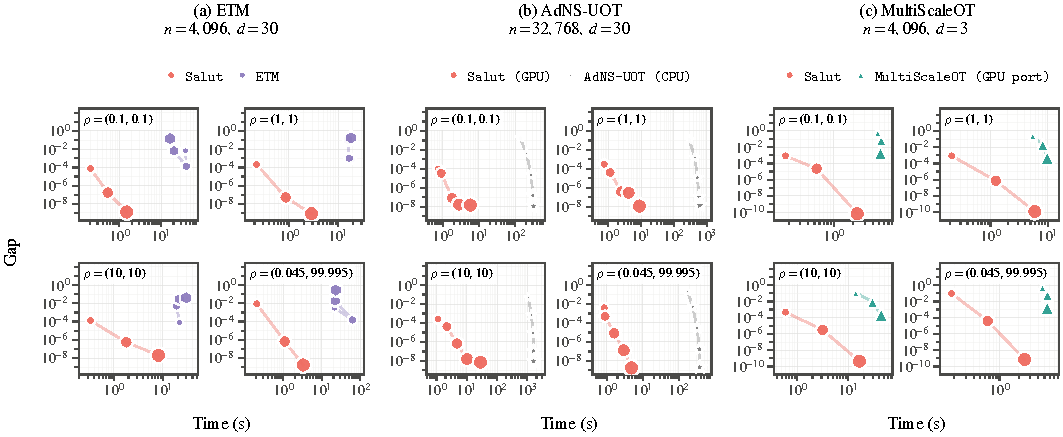
\includegraphics[width=\linewidth]{figures/uot_supplementary_baselines_pilot.pdf}
\caption{\textbf{Supplementary UOT comparisons.}
\ours versus (a) \etm ($n=32{,}768$), (b) \adnsuot ($n=32{,}768$), and (c) \multiscaleot ($n=18{,}432$, $d=3$), with $m=n$.
Larger markers target higher accuracy.
}
\label{fig:uot-supplementary-baselines}
\end{figure}


\subsection{Generality of KL-UOT}
\label{app:uot-generality}

Figure~\ref{fig:uot-generality} evaluates \ours across 28 settings spanning ground costs, datasets, dimensions, and nonuniform reference masses.
While exceeding each baseline's highest achieved accuracy in every panel, \ours achieves geometric mean speedups of $172\times$ over \mm, $107\times$ over \sinkhorn, and $31\times$ over \hellouot.

\begin{figure}[htbp] 
\centering
% CN: 已结束五 seed 批次的 2339/2500 次有效测量；两轮 timing repair（139 cells/695 runs + 43 cells/66 runs）已修复，固定数据见 figures/plot_sources/generality_final_20261120.json。
% EN: Completed five-seed batch with 2339/2500 valid measurements; two timing repairs (139 cells/695 runs + 43 cells/66 runs) were applied; pinned data: figures/plot_sources/generality_final_20261120.json.
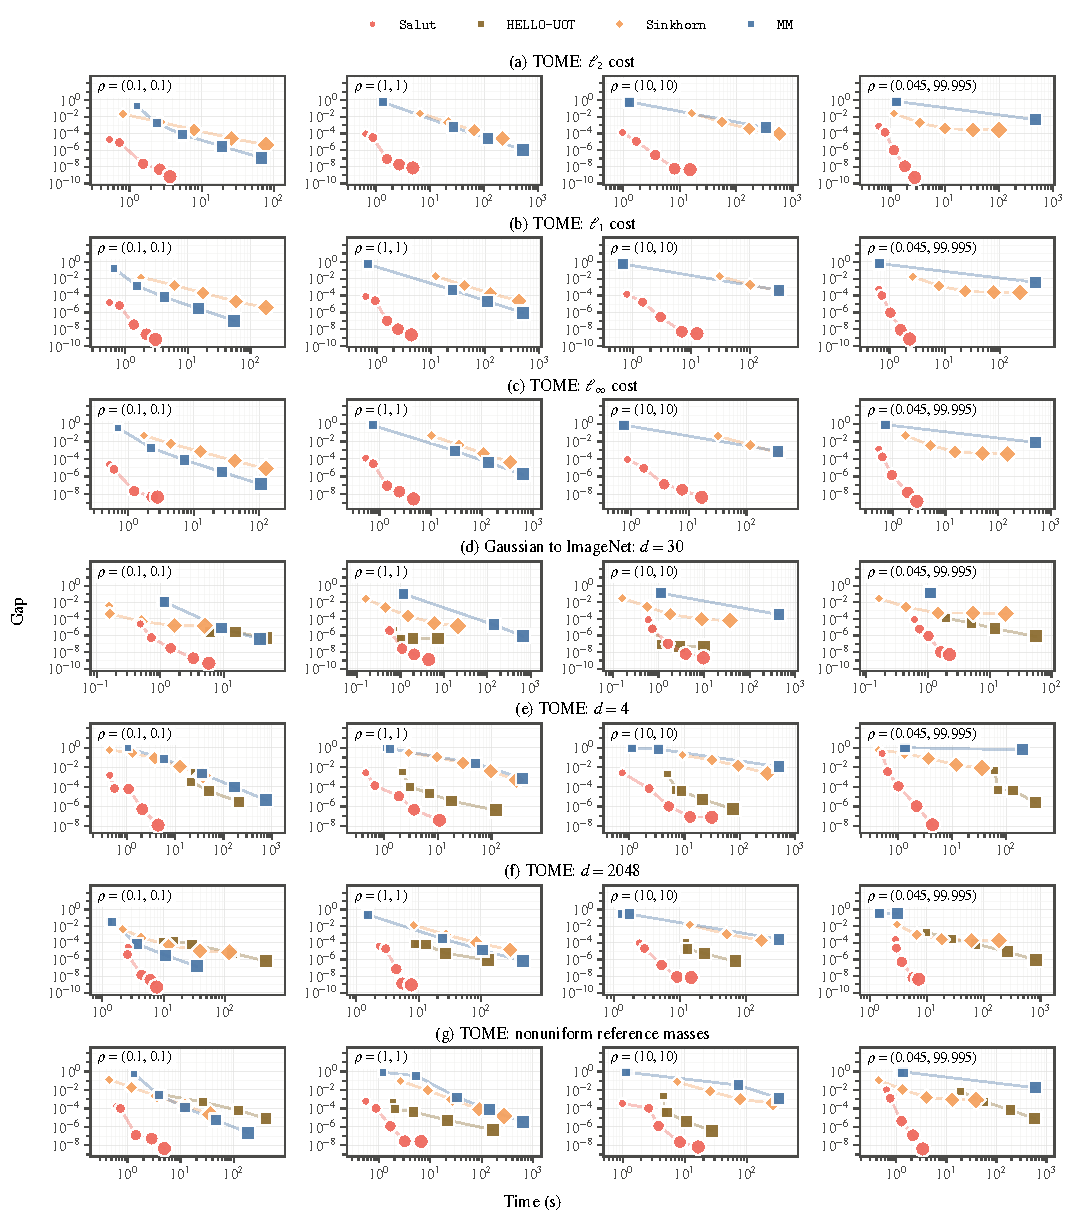
\includegraphics[width=\linewidth]{figures/uot_generality_n16384.pdf}
\caption{\textbf{Runtime--accuracy comparisons across problem settings.}
KL-UOT at $m=n=16{,}384$, with each row varying one setting from the default.
\hellouot appears only in rows (d)--(g), as its released implementation supports only $\ell_2^2$ costs.
Larger markers target higher accuracy.}
\label{fig:uot-generality}
\end{figure}
\subsection{Direct Comparison with \hellouot}
\label{app:hello-uot-comparison}



Figure~\ref{fig:hello-uot-trajectories} breaks down the $m=n=131{,}072$ comparison in Table~\ref{tab:hello-uot-main} by marginal penalty.
Across all four settings, \ours converges faster than \hellouot's initialization alone.
Under moderate and strong symmetric penalties, \hellouot terminates in few outer calls but remains $11.3\times$ and $14.4\times$ slower than \ours, respectively, due to the cost of each balanced-OT oracle call.
Under weak and asymmetric penalties, it requires dozens of outer calls and is $132\times$ and $225\times$ slower, respectively.

\begin{figure}[tb]
\centering
% CN: 与正文 Table 2 同批（20261119_hello_tolerance_table）；按各 seed 取 best-so-far 原问题候选后再按 oracle 调用序号取五 seed 均值，停止后保留最终 incumbent；固定来源见 figures/plot_sources/hello_comparison_final_20261120.json。
% EN: Same batch as Table 2 (20261119_hello_tolerance_table); per-seed best-so-far primal candidates averaged at each oracle-call index, retaining terminal incumbents after stopping; pinned sources: figures/plot_sources/hello_comparison_final_20261120.json.
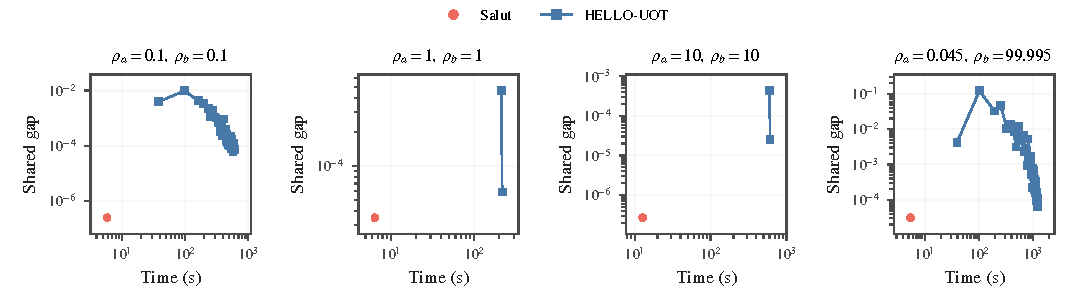
\includegraphics[width=\linewidth]{figures/hello_uot_gap_time_n131072.pdf}
\caption{\textbf{\hellouot trajectories versus final \ours solutions} ($m=n=131{,}072$).
Brown squares trace five-seed mean best-so-far \hellouot primal candidates after initialization and each outer balanced-OT oracle call (inner tolerance $10^{-6}$, outer tolerance $10^{-4}$); the coral dot marks the final \ours solution (tolerance $10^{-6}$).}
\label{fig:hello-uot-trajectories}
\end{figure}

\subsection{Million-Scale Baselines across Penalty Settings}
\label{app:million-scale-additional}

Table~\ref{tab:million-scale-baselines-appendix} extends the $3600$\,s million-point comparison across all four penalty settings.
All baselines exhaust the time budget while retaining gaps over two orders of magnitude larger than \ours.
By contrast, \ours converges within $126$--$170$\,s across all four penalties, maintaining \sharedgap below $3.7\times10^{-5}$ with the lowest GPU memory.

\begin{table}[htbp]
\centering
% CN: 三批基线实测结果和逐次 Gap 计算固定于 tables/million_comparison.json；Salut 来自 scaling_final_20261119.json；表行由 collect.py --million-comparison 生成。
% EN: Three measured baseline batches and per-run gap calculations are pinned in tables/million_comparison.json; Salut comes from scaling_final_20261119.json; rows are generated by collect.py --million-comparison.
\caption{\textbf{Million-point linear-memory baseline comparison across penalty settings} ($m=n=1{,}048{,}576$, $d=30$, Zhuang-ABCA-1$\to$Zhuang-ABCA-2).
Baselines use a soft $3600$\,s budget; $^\dagger$ marks timeouts (reported times are actual runtimes).
Protocol in Appendix~\ref{app:million-baseline-protocol}.}
\label{tab:million-scale-baselines-appendix}
\footnotesize
\setlength{\tabcolsep}{1.5pt}
\begin{tabular*}{\textwidth}{@{\extracolsep{\fill}}lr*{8}{r}@{}}
\toprule
\multirow{2}{*}{Method} & \multirow{2}{*}{\gpumemshort~$\downarrow$} & \multicolumn{2}{c}{$\rho=(0.1,0.1)$} & \multicolumn{2}{c}{$\rho=(1,1)$} & \multicolumn{2}{c}{$\rho=(10,10)$} & \multicolumn{2}{c}{$\rho=(0.045,99.995)$} \\
\cmidrule(lr){3-4}\cmidrule(lr){5-6}\cmidrule(lr){7-8}\cmidrule(lr){9-10}
 & & \runtime~$\downarrow$ & \sharedgap~$\downarrow$ & \runtime~$\downarrow$ & \sharedgap~$\downarrow$ & \runtime~$\downarrow$ & \sharedgap~$\downarrow$ & \runtime~$\downarrow$ & \sharedgap~$\downarrow$ \\
\midrule
% CN: 来源与逐项计算见 million_comparison.json；由 collect.py --million-comparison 生成。
% EN: Sources and per-run calculations: million_comparison.json; generated by collect.py --million-comparison.
\sinkhornonline & 9.10 & $4286.6^{\dagger}$ & $2.00\times10^{-2}$ & $4265.4^{\dagger}$ & $2.17\times10^{-1}$ & $4373.8^{\dagger}$ & $7.73\times10^{-1}$ & $4390.0^{\dagger}$ & $8.37\times10^{-1}$ \\
\ulot & 11.56 & $3652.1^{\dagger}$ & $7.09\times10^{-1}$ & $3649.7^{\dagger}$ & $7.14\times10^{-1}$ & $3619.0^{\dagger}$ & $7.06\times10^{-1}$ & $3620.3^{\dagger}$ & $7.32\times10^{-1}$ \\
\hellouot & 9.10 & $3665.2^{\dagger}$ & $1.25\times10^{-2}$ & $4226.4^{\dagger}$ & $3.62\times10^{-1}$ & $4220.5^{\dagger}$ & $4.84\times10^{-1}$ & $3808.2^{\dagger}$ & $8.40\times10^{-3}$ \\
\ours & \textbf{6.46--6.50} & \textbf{125.5} & $\boldsymbol{1.85\times10^{-5}}$ & \textbf{131.6} & $\boldsymbol{2.95\times10^{-5}}$ & \textbf{169.5} & $\boldsymbol{3.67\times10^{-5}}$ & \textbf{128.7} & $\boldsymbol{3.40\times10^{-5}}$ \\
\bottomrule

\end{tabular*}
\end{table}


% CN: 分析实验附录；占位数据与实测结果必须显式区分。
% EN: Analysis-exper iment appendix; placeholder data must be explicitly distinguished from measurements.
\subsection{Accuracy across Entropic Strengths}
\label{app:entropic-epsilon-accuracy}

Figure~\ref{fig:entropic-epsilon-accuracy} tests how accurately \ourssparsink approximates the dense entropic solution across seven entropic strengths $\varepsilon\in[10^{-3.5},10^{-2.5}]$ at $m=n=16{,}384$, using the fixed support budget and tolerance $10^{-6}$ against an independent FP64 \ottonline reference (threshold $10^{-8}$) at each $\varepsilon$.
For entropic UOT comparisons, we evaluate the full entropic primal $P_\varepsilon$ against the independent reference dual bound $D_{\varepsilon,\mathrm{ref}}$ via the normalized shared gap
\begin{equation}
\entropicgap=\frac{P_\varepsilon-D_{\varepsilon,\mathrm{ref}}}{\max\{|P_\varepsilon|,|D_{\varepsilon,\mathrm{ref}}|,10^{-15}\}}.
\label{eq:entropic-evaluation-gap}
\end{equation}
Here we additionally report the entrywise relative coupling error $e_{\mathbf X}$ and the reference mass fraction $e_{\mathrm{out}}$ omitted outside the reconstructed support $\mathcal N$:
\begin{equation*}
e_{\mathbf X} = \frac{\|\mathbf X-\mathbf X_{\mathrm{ref}}\|_1}{\|\mathbf X_{\mathrm{ref}}\|_1}, \qquad
e_{\mathrm{out}} = \frac{\sum_{(i,j)\notin\mathcal N}(X_{\mathrm{ref}})_{ij}}{\sum_{ij}(X_{\mathrm{ref}})_{ij}},
\end{equation*}
where $e_{\mathrm{out}}$ lower-bounds $e_{\mathbf X}$ since $\mathbf X$ vanishes outside $\mathcal N$.
Across all four penalty settings, approximation accuracy improves rapidly as $\varepsilon$ decreases: at $\varepsilon=10^{-3}$, the shared gap is $2.26$--$2.41\times10^{-7}$, $e_{\mathbf X}$ is $9.83\times10^{-5}$--$2.04\times10^{-4}$, and $e_{\mathrm{out}}$ is $2.42$--$3.91\times10^{-5}$, with all three metrics smaller still for $\varepsilon<10^{-3}$.

\begin{figure}[tb]
\centering
% CN: 三指标五-seed 均值曲线来自 paper_experiments_uot/entropic_epsilon_accuracy/results/20261117_paper_data_entropic_epsilon_accuracy/{epsilon_aggregate.json,config.json}；固定输入及来源 SHA256 见 figures/plot_sources/entropic_epsilon_sparse_20261120.json，重画入口 scripts/plot_entropic_epsilon_accuracy.py；140/140 有效，仅 sparse readout。
% EN: Five-seed mean metric curves use paper_experiments_uot/entropic_epsilon_accuracy/results/20261117_paper_data_entropic_epsilon_accuracy/{epsilon_aggregate.json,config.json}; pinned inputs and source SHA256 are in figures/plot_sources/entropic_epsilon_sparse_20261120.json. Redraw with scripts/plot_entropic_epsilon_accuracy.py; all 140 sparse observations are valid.
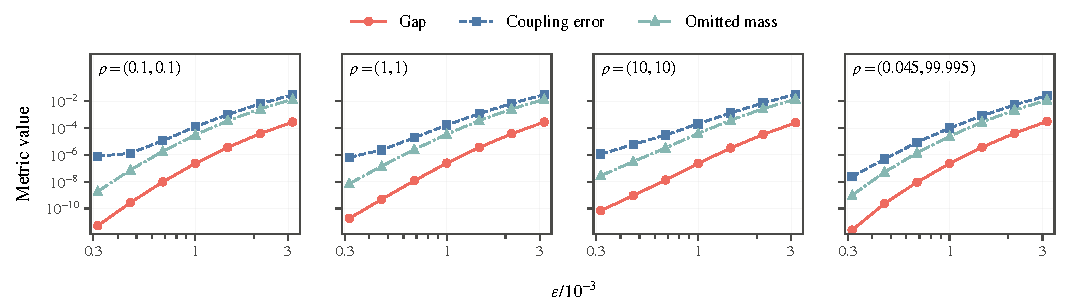
\includegraphics[width=\linewidth]{figures/entropic_epsilon_sparse_accuracy.pdf}
\caption{\textbf{Sparse entropic UOT accuracy across entropic strengths} ($m=n=16{,}384$).
Each point evaluates the returned sparse coupling against an independent FP64 \ottonline reference at the same $\varepsilon$.}
\label{fig:entropic-epsilon-accuracy}
\end{figure}

\subsection{UFGW Solver Trajectories}
\label{app:ufgw-solver-trajectories}

Figure~\ref{fig:ufgw-objective-time} shows the objective--time trajectories from the same runs as Table~\ref{tab:ufgw-solvers}, evaluated in CPU FP64 on the common two-coupling objective
\begin{equation}
\ufgwobj(\mathbf P,\mathbf Q) = \mathcal F_0(\mathbf P,\mathbf Q) + \varepsilon\,\KL(\mathbf P\otimes\mathbf Q\,|\,(\mathbf a\otimes\mathbf b)\otimes(\mathbf a\otimes\mathbf b)),
\label{eq:ufgw-eval-objective}
\end{equation}
where $\mathcal F_0(\mathbf P,\mathbf Q)$ is the unregularized objective in~\eqref{eq:ufgw-relaxation}.
Our variants complete all ten sweeps $30.0\times$ faster than \bcdmm at $\varepsilon=0$ and $5.8\times$ faster than \bcdsinkhorn at $\varepsilon=10^{-3}$, matching \bcdsinkhorn's objective at $\varepsilon=10^{-3}$ and attaining a lower objective than \bcdmm at $\varepsilon=0$.

\begin{figure*}[htb]
\centering
% CN: 左右两图均来自 paper_experiments_uot/ufgw_solver_comparison/results/20261117_paper_data_ufgw_solver_comparison/cases/*/{shuttle,pot}_repeat0/trajectory.json（seeds 0--4 按 sweep 取五-seed 均值）；固定轨迹与来源 SHA256 见 figures/plot_sources/ufgw_solver_comparison_20261120.json。
% EN: Both panels use five-seed sweep-averaged trajectories from paper_experiments_uot/ufgw_solver_comparison/results/20261117_paper_data_ufgw_solver_comparison/cases/*/{shuttle,pot}_repeat0/trajectory.json (seeds 0--4); pinned trajectories and source SHA256: figures/plot_sources/ufgw_solver_comparison_20261120.json.
\begin{subfigure}[t]{0.49\textwidth}
\centering
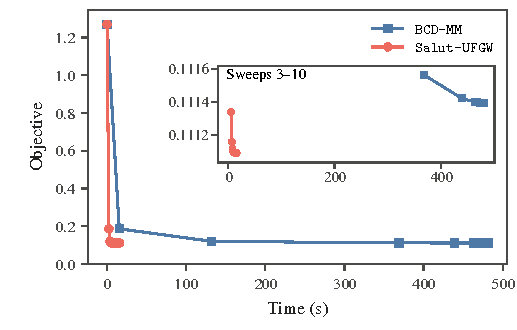
\includegraphics[width=\linewidth]{figures/ufgw_objective_time_eps0.pdf}
\caption{$\varepsilon=0$.}
\end{subfigure}\hfill
\begin{subfigure}[t]{0.49\textwidth}
\centering
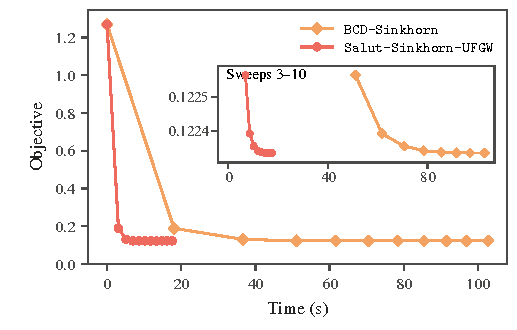
\includegraphics[width=\linewidth]{figures/ufgw_objective_time_eps0.001.pdf}
\caption{$\varepsilon=10^{-3}$.}
\end{subfigure}
\caption{\textbf{UFGW objective--time trajectories} on STARmap well05--well11 ($m=n=16{,}384$, $d=30$, $\alpha=0.4$, $\rho_a=\rho_b=0.1$).
Markers denote initialization and ten complete sweeps, averaged across five seeds at each sweep.}
\label{fig:ufgw-objective-time}
\end{figure*}


\subsection{Temporal Transport Timing}
\label{app:temporal-timing}
\begin{figure}[htb]
\centering
% CN: 分项数据来自 paper_experiments_uot/moscot_time/results/20261117_paper_data_moscot_time/summary_table.csv；固定绘图输入与 SHA256 见 figures/plot_sources/moscot_time_20261120.json，由 moscot_time/collect.py::plot 重画。
% EN: Timing data originate from paper_experiments_uot/moscot_time/results/20261117_paper_data_moscot_time/summary_table.csv; pinned inputs and SHA256 hashes are in figures/plot_sources/moscot_time_20261120.json, redrawn via moscot_time/collect.py::plot.
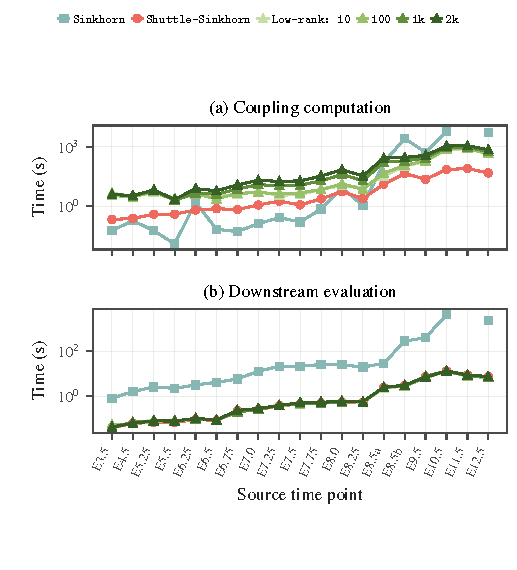
\includegraphics[width=\linewidth]{figures/moscot_time_runtime.pdf}
\caption{\textbf{Temporal transport timing breakdown} across the 19 mouse-embryogenesis time pairs (seed 42).
(a) Coupling computation; (b) downstream evaluation.}
\label{fig:temporal-timing-breakdown}
\end{figure}
Figure~\ref{fig:temporal-timing-breakdown} separates coupling computation from the moscot downstream evaluation pipeline across the 19 time pairs of Figure~\ref{fig:temporal-runtime}.
Downstream evaluation uses native OTT GPU operators for full-rank \sinkhorn and \ulot, and CPU CSR operations through the same moscot API for \ourssparsink; even on CPU, \ourssparsink matches \ulot's evaluation speed (and is one to two orders of magnitude faster than full-rank \sinkhorn on late stages) while substantially accelerating coupling computation.
% CN: 统计来自 paper_experiments_uot/moscot_time/results/20261117_paper_data_moscot_time/{summary.csv,summary_table.csv}；114/114 项已完成（seed 42）。
% EN: Statistics come from paper_experiments_uot/moscot_time/results/20261117_paper_data_moscot_time/{summary.csv,summary_table.csv}, with 114/114 configurations complete (seed 42).


\section{Component and Mechanism Analysis}
\label{app:component-mechanism-analysis}

\subsection{Hyperparameter Sensitivity}
\label{app:uot-parameter-sensitivity}

Table~\ref{tab:uot-parameter-sensitivity} varies the hierarchy split factor $s$, dual-assignment budget $\kappa$, pricing budget $\gamma$, and support budget factor $\beta$ one at a time around the default $(s,\kappa,\gamma,\beta)=(4,16,2,10)$ at $m=n=262{,}144$ (coarsest threshold $256$, KKT tolerance $10^{-6}$).
Across all four parameters and penalty settings, runtime stays within $0.94$--$1.52\times$ of the default and memory remains low (scaling linearly with $\kappa$ as expected), showing that \ours is insensitive to hyperparameter choices around the default.

\begin{table}[tb]
\centering
% CN: 全部耗时与显存均值来自 paper_experiments_uot/parameter_sensitivity/results/20261117_paper_data_parameter_sensitivity/summary_table.json；原始指标为同批次 cases/*/*/metrics.json；n=262144，五 seed（seeds 42--46），180/180 成功（含 refinement_forcing_check=True 与 J=64）；固定汇总与 SHA256 见 figures/plot_sources/parameter_sensitivity_20261120.json。四块共享每组 penalty 的 baseline，显存为 peak_gpu_memory_mib / 1024。
% EN: All mean runtimes and memory measurements come from paper_experiments_uot/parameter_sensitivity/results/20261117_paper_data_parameter_sensitivity/summary_table.json, with raw metrics in cases/*/*/metrics.json; n=262144, five seeds (42--46), 180/180 successful runs (refinement_forcing_check=True, J=64); pinned aggregates and SHA256: figures/plot_sources/parameter_sensitivity_20261120.json. Blocks share each penalty's baseline, and memory is peak_gpu_memory_mib / 1024.
\caption{\textbf{Hyperparameter sensitivity across marginal penalties} ($m=n=262{,}144$, KKT tolerance $10^{-6}$).
Each block varies one parameter; lower is better, with bold and underlined entries marking the best and second-best displayed values per block and penalty.}
\label{tab:uot-parameter-sensitivity}
\footnotesize
\setlength{\tabcolsep}{3pt}
\begin{tabular}{@{}l cc cc cc cc@{}}
\toprule
\multirow{2}{*}{Variant} & \multicolumn{2}{c}{$(0.1,0.1)$} & \multicolumn{2}{c}{$(1,1)$} & \multicolumn{2}{c}{$(10,10)$} & \multicolumn{2}{c}{$(0.045,99.995)$} \\
\cmidrule(lr){2-3}\cmidrule(lr){4-5}\cmidrule(lr){6-7}\cmidrule(lr){8-9}
 & \runtime~$\downarrow$ & \gpumem~$\downarrow$ & \runtime~$\downarrow$ & \gpumem~$\downarrow$ & \runtime~$\downarrow$ & \gpumem~$\downarrow$ & \runtime~$\downarrow$ & \gpumem~$\downarrow$ \\
\midrule
\multicolumn{9}{l}{\textit{(a) Hierarchy split factor $s$ ($\kappa=16,\gamma=2,\beta=10$)}} \\
$s=2$ & 17.91 & \textbf{1.625} & 21.84 & \textbf{1.600} & \underline{30.45} & \textbf{1.589} & 18.73 & \textbf{1.637} \\
$s=4$ & \textbf{13.76} & \underline{1.647} & \textbf{15.95} & \underline{1.629} & \textbf{26.32} & 1.612 & \textbf{14.09} & \underline{1.650} \\
$s=8$ & \underline{14.67} & 1.683 & \underline{16.91} & 1.664 & 31.74 & \underline{1.611} & \underline{14.73} & 1.696 \\
\midrule
\multicolumn{9}{l}{\textit{(b) Dual-assignment budget $\kappa$ ($s=4,\gamma=2,\beta=10$)}} \\
$\kappa=8$ & \underline{15.25} & \textbf{1.039} & \underline{18.83} & \textbf{1.024} & \underline{26.60} & \textbf{1.021} & \underline{15.63} & \textbf{1.042} \\
$\kappa=16$ & \textbf{13.76} & \underline{1.647} & \textbf{15.95} & \underline{1.629} & \textbf{26.32} & \underline{1.612} & \textbf{14.09} & \underline{1.650} \\
$\kappa=32$ & 16.80 & 3.063 & 22.93 & 3.009 & 39.98 & 2.997 & 17.23 & 3.071 \\
\midrule
\multicolumn{9}{l}{\textit{(c) Pricing budget $\gamma$ ($s=4,\kappa=16,\beta=10$)}} \\
$\gamma=1$ & \textbf{12.99} & \textbf{1.647} & \textbf{15.84} & \textbf{1.629} & \textbf{25.18} & \underline{1.613} & \textbf{13.24} & \textbf{1.650} \\
$\gamma=2$ & \underline{13.76} & \textbf{1.647} & \underline{15.95} & \textbf{1.629} & \underline{26.32} & \textbf{1.612} & \underline{14.09} & \textbf{1.650} \\
$\gamma=4$ & 14.81 & \textbf{1.647} & 17.93 & \textbf{1.629} & 27.16 & \underline{1.613} & 14.91 & \textbf{1.650} \\
\midrule
\multicolumn{9}{l}{\textit{(d) Support budget factor $\beta$ ($s=4,\kappa=16,\gamma=2$)}} \\
$\beta=5$ & 13.85 & \textbf{1.637} & \textbf{15.88} & \textbf{1.629} & \underline{25.67} & \textbf{1.600} & \textbf{13.85} & \textbf{1.640} \\
$\beta=10$ & \underline{13.76} & \underline{1.647} & 15.95 & \textbf{1.629} & 26.32 & \underline{1.612} & 14.09 & \underline{1.650} \\
$\beta=20$ & \textbf{13.67} & 1.656 & \underline{15.91} & \textbf{1.629} & \textbf{25.64} & 1.650 & \underline{13.98} & 1.659 \\
\bottomrule
\end{tabular}
\end{table}

\subsection{Runtime Breakdown}
\label{app:runtime-breakdown}

\begin{figure}[tb]
\centering
% CN: 四档 MERFISH 规模、四组 penalty、五 seed 共 80 个正式 profile；原始来源、SHA256、阶段耗时及扫描次数见 figures/plot_sources/runtime_breakdown_20261119.json；复现入口 scripts/plot_runtime_breakdown.py。
% EN: Eighty formal MERFISH profiles across four sizes, four penalties and five seeds; sources, SHA256, phase timings and scan counts: figures/plot_sources/runtime_breakdown_20261119.json; redraw with scripts/plot_runtime_breakdown.py.
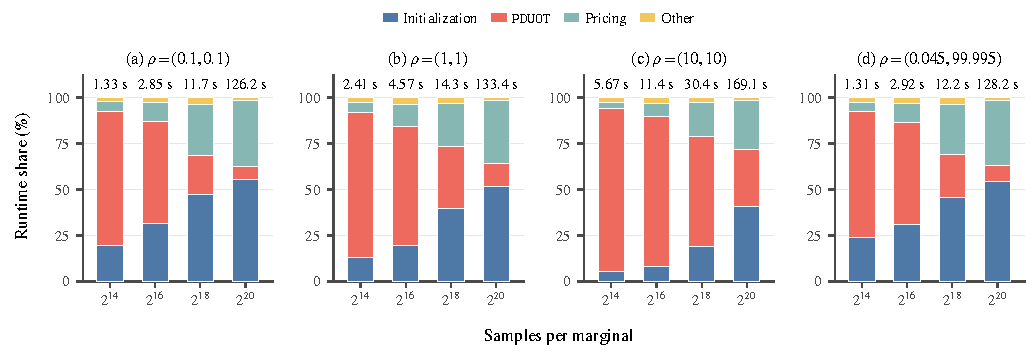
\includegraphics[width=\linewidth]{figures/uot_runtime_breakdown.pdf}
\caption{\textbf{Runtime breakdown of \ours} on MERFISH instances ($m=n$, KKT tolerance $10^{-6}$).
Bars show each phase's share of mean total runtime (bar-top labels); Other includes support maintenance.}
\label{fig:uot-runtime-breakdown}
\end{figure}

Figure~\ref{fig:uot-runtime-breakdown} decomposes \ours's runtime across problem sizes.
At moderate scale ($n=65{,}536$), \subsolver accounts for $55$--$82\%$ of total runtime, highlighting the importance of its efficiency to overall performance.
At one million points per marginal, its share falls to $7$--$31\%$, and initialization and pricing, both involving $O(n^2d)$ pairwise computations, become the dominant costs.
Accelerating these pairwise scans while preserving linear memory and exact optimality certification is therefore a natural direction for future work.


\subsection{Convergence Safeguards}
\label{app:pduot-weight-budget-experiment}

Figure~\ref{fig:pduot-weight-budget} measures the iteration cost of the summable weight-update budget~\eqref{eq:pduot-weight-budget} and the refinement safeguard in \checkstop on complete \ours solves ($m=n=65{,}536$, $p=1.01$, KKT tolerance $10^{-6}$).
For each seed, we sum inner iterations across all hierarchy levels and all four penalty pairs.
For $J\geq4$ (including the default $J=64$), the weight budget has no effect on iteration counts; even at $J=1$ and $J=2$, mean total iterations increase by only $2.72\%$ and $0.62\%$, respectively.
Likewise, the refinement safeguard at $J=64$ adds only $0.077\%$ to mean total iterations.
Thus, the default budget and refinement safeguard enforce our theoretical convergence conditions at negligible iteration overhead.

\begin{figure}[tb]
\centering
% CN: 数据来源：paper_experiments_uot/primal_weight_budget/results/20261115_224339_safeguard_my4090/summary.json；180/180 个测量成功，复用 20261115_195720_J1_my4090 的 160 个预算测量，新增 20 个关闭 safeguard 的测量，RTX 4090，固定 p=1.01。
% EN: Source: paper_experiments_uot/primal_weight_budget/results/20261115_224339_safeguard_my4090/summary.json; all 180 observations succeeded, reusing 160 budget measurements from 20261115_195720_J1_my4090 and adding 20 safeguard-disabled measurements on RTX 4090 with fixed p=1.01.
% CN: 固定汇总与原始指标 SHA256：figures/plot_sources/convergence_safeguards_20261115.json；复现入口：paper_experiments_uot/primal_weight_budget/collect.py --batch-id 20261115_224339_safeguard_my4090。
% EN: Frozen summary and raw-metric SHA256: figures/plot_sources/convergence_safeguards_20261115.json; reproduce with paper_experiments_uot/primal_weight_budget/collect.py --batch-id 20261115_224339_safeguard_my4090.
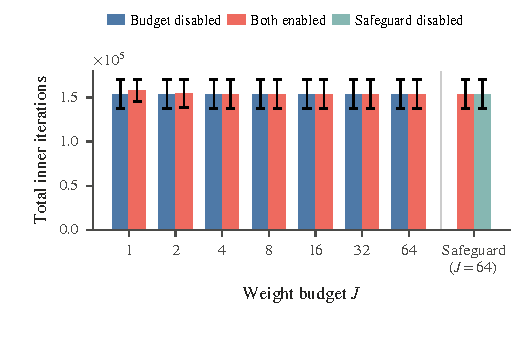
\includegraphics[width=3.45in]{figures/uot_primal_weight_budget.pdf}
\caption{\textbf{Iteration cost of convergence safeguards} ($m=n=65{,}536$, $p=1.01$).
Total inner iterations per seed summed over all levels and four penalty pairs; the rightmost pair compares removing the refinement safeguard at $J=64$.
Bars show means and error bars denote sample standard deviations over five seeds.}
\label{fig:pduot-weight-budget} 
\end{figure}


\subsection{Support Sparsification}
\label{app:sparsification-experiment}

Figure~\ref{fig:uot-sparsification-scaling} evaluates the two-pass \sparsify procedure on cyclic sparse supports with $m=n\in[2^{10},2^{20}]$ across four ground costs and three feature dimensions.
All 360 runs satisfy the output-support cap, with maximum absolute marginal errors below $1.1\times10^{-18}$ and objective errors below $1.1\times10^{-11}$ for both KL and $\ell_2^2$ penalties.
Sparsification time scales nearly linearly with $n$ and is insensitive to feature dimension and ground cost.

\begin{figure}[tb]
\centering
% CN: 图源 paper_experiments/support_sparsification_uot/results/support_sparsification_uot_scaling.pdf；绘图输入为同目录 summary.json，原始记录为 records.jsonl。
% EN: Figure source: paper_experiments/support_sparsification_uot/results/support_sparsification_uot_scaling.pdf; plotting input: summary.json, raw measurements: records.jsonl in the same directory.
% CN: 由 paper_experiments/support_sparsification_uot/plot_scaling.py 生成；正文数值核验使用全部 360 条 records.jsonl 记录。
% EN: Generated by paper_experiments/support_sparsification_uot/plot_scaling.py; numerical checks in the text use all 360 records in records.jsonl.
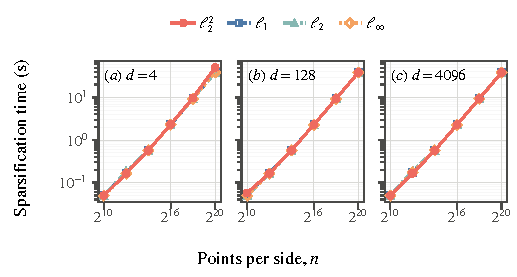
\includegraphics[width=0.52\linewidth]{figures/support_sparsification_uot_scaling.pdf}
\caption{\textbf{UOT support-sparsification scaling} on cyclic sparse supports.
Time covers both CPU cycle-cancellation passes and convex mixing; values are medians over five repeated timings per fixed input.}
% \xwz{SEED COVERAGE: Five timings reuse each fixed input and are summarized by medians. They are not five independent seeds; retain this exception or rerun independent inputs before changing the statistical claim.}
\label{fig:uot-sparsification-scaling}
\end{figure}

% CN: 共享侧响应稳定性及其与势传播的联系；辅助预测分析已归档。
% EN: Shared-side response stability and its link to potential propagation; auxiliary prediction analysis is archived.
\subsection{Inter-Level Response Stability}
\label{app:uot-hierarchy-stability}

Consider two KL-UOT problems sharing target locations, positive reference weights $\mathbf b$, and penalty $\rho_b>0$, while their source locations, positive source weights, or positive source penalties may differ.
Costs are finite, and the coupling has no entropic regularization.
For a target potential $\mathbf g$, define its normalized marginal response by
\begin{equation*}
p_j(\mathbf g)=\frac{b_j e^{-g_j/\rho_b}}{\sum_k b_k e^{-g_k/\rho_b}}.
\end{equation*}
This response is invariant under scalar translation of $\mathbf g$.
We measure response differences by $H^2(p,z)=\sum_j(\sqrt{p_j}-\sqrt{z_j})^2$.
The argument applies to adjacent hierarchy levels sharing the target side; exchanging the marginals covers the other direction.

For two source instances with a common target set, take their union as the source index set and define the rectangular cost oscillation
$$\Gamma=\max_{i,i',j,j'}|C_{ij}-C_{ij'}-C_{i'j}+C_{i'j'}|.$$

\begin{proposition}[Shared-side response stability]
\label{prop:uot-hierarchy-stability}
\label{prop:uot-hierarchy-interaction}
Let $p^0,p^1$ be the normalized optimal target marginals of any two such source instances with the same $b$ and $\rho_b$.
Then
$$H^2(p^0,p^1)\leq2\left[1-\operatorname{sech}\!\left(\frac{\Gamma}{4\rho_b}\right)\right]\leq\frac{\Gamma^2}{16\rho_b^2}.$$
For squared Euclidean cost, $\Gamma\leq2\operatorname{diam}(S)\operatorname{diam}(T)$, where $S$ contains both source sets and $T$ is the common target set.
For separable cost $C_{ij}=u_i+v_j$, the target-response shape is exactly $p_j\propto b_j e^{-v_j/\rho_b}$ and is unchanged by source subsampling or source reweighting.
The first bound is sharp over pairs of source instances.
\end{proposition}
\begin{proof}
Positive optimal target marginals imply $g_j=\min_i(C_{ij}-f_i)$.
Thus each difference $g_j-g_{j'}$ lies between the minimum and maximum of $C_{ij}-C_{ij'}$ over the available source indices.
Using the union of both source sets gives $\operatorname{osc}(g^1-g^0)\leq\Gamma$.
The normalized log-likelihood ratio therefore has oscillation at most $D=\Gamma/\rho_b$.

For completeness, let $x_j=\sqrt{p^1_j/p^0_j}\in[\alpha,\beta]$, with $\beta/\alpha\leq e^{D/2}$.
Since $\mathbb E_{p^0}x^2=1$ and $(x-\alpha)(x-\beta)\leq0$,
$$\mathbb E_{p^0}x\geq\frac{1+\alpha\beta}{\alpha+\beta}\geq\operatorname{sech}(D/4).$$
The final inequality follows by minimizing over $\alpha$ at fixed $\beta/\alpha$.
The affinity identity $H^2=2-2\mathbb E x$ proves the first bound.
The inequality $2(1-\operatorname{sech} t)\leq t^2$ proves the second.
For quadratic cost the rectangular difference is $-2(s_i-s_{i'})^\top(t_j-t_{j'})$.
If $\Gamma=0$, the bound gives exact inheritance; the displayed separable response also follows directly from the optimality conditions.
For sharpness, take two singleton source instances whose costs to two equally weighted targets are $(0,\Gamma/2)$ and $(\Gamma/2,0)$.
Their normalized target responses attain $H^2=2[1-\operatorname{sech}(\Gamma/(4\rho_b))]$.
\end{proof}

The bound concerns optimal response shapes and can be conservative on large supports; it provides neither a sampling rate nor a warm-start iteration bound.

\begin{corollary}[Weighted potential stability]
\label{cor:uot-hierarchy-weighted-potentials}
For any two finite target potentials $g^0,g^1$ with a common positive reference $b$ and penalty $\rho_b>0$, define
$$Z_s=\sum_j b_j e^{-g_j^s/\rho_b},\qquad p_j^s=\frac{b_j e^{-g_j^s/\rho_b}}{Z_s},\qquad s\in\{0,1\},$$
and remove scalar translations by setting $\bar g^s=g^s+\rho_b\log Z_s\,\mathbf1$.
Then
\begin{equation*}
\sum_j\sqrt{p_j^0p_j^1}\,(\bar g_j^1-\bar g_j^0)^2\leq4\rho_b^2H^2(p^0,p^1).
\end{equation*}
No uniform positive lower bound on the response entries is required.
\end{corollary}
\begin{proof}
Writing $\delta_j=\bar g_j^1-\bar g_j^0$, the response identity gives $\delta_j=-\rho_b\log(p_j^1/p_j^0)$.
Consequently,
$$H^2(p^0,p^1)=4\sum_j\sqrt{p_j^0p_j^1}\,\sinh^2\!\left(\frac{\delta_j}{4\rho_b}\right)\geq\frac{1}{4\rho_b^2}\sum_j\sqrt{p_j^0p_j^1}\,\delta_j^2,$$
where the inequality uses $|\sinh x|\geq|x|$.
\end{proof}

The estimate connects response stability to dual propagation by controlling the aligned potentials with weights that emphasize coordinates carrying mass in both responses.
Coordinates with vanishing response weight may still have large potential differences, so the estimate does not imply uniform coordinatewise stability.



\section{$\ell_2^2$ Marginal Penalties}
\label{app:l2-penalty}

\subsection{Model and Solver Adaptation}
\label{app:l2-adaptation}

The active-support construction and two-sided PDHG formulation also apply to $\ell_2^2$ marginal penalties.
For $\mathbf r=\mathbf X\mathbf1$ and $\mathbf q=\mathbf X^\top\mathbf1$, define
\begin{equation*}
\Phi_2(\mathbf X)=\langle\mathbf C,\mathbf X\rangle+\frac{\rho_a}{2}\|\mathbf r-\mathbf a\|_2^2+\frac{\rho_b}{2}\|\mathbf q-\mathbf b\|_2^2,\qquad \mathbf X\geq0.
\end{equation*}
Throughout this section, the discrete problem is finite, costs are finite and nonnegative, reference masses are positive, and $\rho_a,\rho_b>0$.
Transported marginals may vanish.

\paragraph{Dual and proximal map.}
For one node, let $H_{\rho,h}(r)=\rho(r-h)^2/2+\iota_{\mathbb R_+}(r)$.
Its conjugate and proximal map are
\begin{equation*}
H_{\rho,h}^*(y)=\frac{[y+\rho h]_+^2}{2\rho}-\frac{\rho h^2}{2},\qquad
\operatorname{prox}_{sH_{\rho,h}^*}(u)=
\begin{cases}
u,&u\leq-\rho h,\\
(u-sh)/(1+s/\rho),&u>-\rho h.
\end{cases}
\end{equation*}
Writing $d_{\rho,h}(f)=-H_{\rho,h}^*(-f)$, the restricted dual maximizes
\begin{equation*}
D_2(\mathbf f,\mathbf g)=\sum_i d_{\rho_a,a_i}(f_i)+\sum_j d_{\rho_b,b_j}(g_j)
\quad\text{subject to}\quad f_i+g_j\leq C_{ij},\quad(i,j)\in\mathcal N.
\end{equation*}
The marginal responses are $[\mathbf a-\mathbf f/\rho_a]_+$ and $[\mathbf b-\mathbf g/\rho_b]_+$.

\paragraph{Primal-consistent readout.}
At a KKT checkpoint, a nonnegative candidate $\mathbf x$ admits the readout
\begin{equation*}
\mathbf f^{\mathbf x}=\rho_a(\mathbf a-\mathbf r),\qquad
\mathbf g^{\mathbf x}=\rho_b(\mathbf b-\mathbf q).
\end{equation*}
This readout satisfies the marginal equations exactly, including at zero marginals.
It changes only the candidate output; the internal iterates, restart anchors and weights are retained.
For $s_e=c_e-f_i^{\mathbf x}-g_j^{\mathbf x}$, choose $\lambda_e=0$ when $x_e>0$ and $\lambda_e=[s_e]_+$ otherwise, and recompute the restricted certificate.
As mapped iterates converge, these readouts converge to a restricted KKT point, so every positive restricted tolerance is attainable.
The readout is also used for full-space pricing.

\paragraph{Coordinate gain and stopping.}
The primal-consistent score and its exact one-edge gain are
\begin{equation*}
\sigma_{ij}^{\mathbf x}=\rho_a(a_i-r_i)+\rho_b(b_j-q_j)-C_{ij},\qquad
g_{ij}(\mathbf x)=\frac{[\sigma_{ij}^{\mathbf x}]_+^2}{2(\rho_a+\rho_b)}.
\end{equation*}
For $\sigma_{ij}^{\mathbf x}\geq\delta>0$, the gain is at least $\Gamma_\delta=\delta^2/[2(\rho_a+\rho_b)]$.
The readout makes the one-sided marginal-gradient error $\Omega$ zero.
For a fixed padded anchor $\mathbf x^0$, the exact objective decrease can be evaluated without dense costs:
\begin{equation*}
\Delta_2=\mathbf c_{\mathcal N}^{\top}(\mathbf x^0-\mathbf x)
+\frac{\rho_a}{2}\langle\mathbf r^0-\mathbf r,\mathbf r^0+\mathbf r-2\mathbf a\rangle
+\frac{\rho_b}{2}\langle\mathbf q^0-\mathbf q,\mathbf q^0+\mathbf q-2\mathbf b\rangle.
\end{equation*}
Use this decrease in the output conditions of Theorem~\ref{thm:refinement-explicit}, with $\Phi_2$ and the gains above.
These tests use $O(|\mathcal N|+m+n)$ work and linear storage.

\subsection{Convergence Guarantees}
\label{app:l2-convergence}

The following results assume exact arithmetic and exact proximal evaluations.

\begin{theorem}[PDUOT with $\ell_2^2$ penalties]
\label{thm:l2-pduot}
Fix a nonempty active support and positive diagonal base steps with $\|\overline{\mathbf D}_y^{1/2}\mathbf A_{\mathcal N}\overline{\mathbf D}_x^{1/2}\|_2<1$.
Use the reflected Halpern iteration, mapped-point restarts, bounded positive weights and summable log-weight update budget of Theorem~\ref{thm:pduot-global}.
Then the iterates and mapped points converge globally to a restricted KKT point.
With the bounded-gap residual-reduction checks and refreshed baselines specified in Theorem~\ref{thm:pduot-local}, convergence is locally R-linear in PDHG evaluations.
\end{theorem}

\begin{proof}
The primal objective is coercive on the nonnegative orthant: writing $M=\|\mathbf x\|_1$, the two marginal totals equal $M$, and $\|\mathbf r\|_2^2\geq M^2/m$, $\|\mathbf q\|_2^2\geq M^2/n$.
Thus an optimum exists.
The differentiable quadratic objective over $\mathbf x\geq0$ supplies finite KKT potentials $\mathbf f^\star=\rho_a(\mathbf a-\mathbf r^\star)$ and $\mathbf g^\star=\rho_b(\mathbf b-\mathbf q^\star)$, including at zero marginals.

Let $G_2$ be the sum of the node functions above and define
\begin{equation*}
\mathcal M_2(\mathbf x,\mathbf y)=
\begin{pmatrix}
\mathbf c+\mathbf A_{\mathcal N}^{\top}\mathbf y+N_{\mathbb R_+^{|\mathcal N|}}(\mathbf x)\\
\nabla G_2^*(\mathbf y)-\mathbf A_{\mathcal N}\mathbf x
\end{pmatrix}.
\end{equation*}
This mapping is maximally monotone.
The PDHG map is its preconditioned resolvent under the same metric as in Appendix~\ref{app:pduot-global}.
The metric comparison and epoch descent arguments therefore give global convergence without any positive-marginal assumption.

For the local rate, $\nabla G_2^*$ is piecewise affine and the graph of the orthant normal cone is a finite union of polyhedra.
Hence the graph of $\mathcal M_2$ is a finite union of polyhedra.
Hoffman's bound on each graph piece containing $(\mathbf z^\star,0)$ gives a local error bound
\begin{equation*}
\operatorname{dist}(\mathbf z,\mathcal M_2^{-1}(0))\leq\kappa\operatorname{dist}(0,\mathcal M_2(\mathbf z)).
\end{equation*}
Indeed, impose the additional linear equation $\mathbf v=0$ on each such piece of $(\mathbf z,\mathbf v)$ and take the maximum of the finitely many Hoffman constants.
Closed graph pieces not containing $(\mathbf z^\star,0)$ are excluded in a sufficiently small neighborhood.
Residuals outside that neighborhood satisfy a local bound by comparison with $\mathbf z^\star$.
The resolvent argument transfers this error bound to fixed-point sharpness.
The proof in Appendix~\ref{app:pduot-restart} then establishes the stated local rate.
\end{proof}

\begin{theorem}[Finite $\ell_2^2$ refinement]
\label{thm:l2-refinement}
Use exact bidirectional top-$\gamma$ pricing with $\gamma\geq1$, pruning that retains positive-flow and newly priced edges, and sparsification preserving transported marginals and transport cost.
Suppose restricted calls use the convergent solver of Theorem~\ref{thm:l2-pduot}, the primal-consistent readout, and the output conditions above.
Then refinement terminates in finitely many rounds at any prescribed positive restricted and full-space tolerances.
With exact restricted solves and exact full-space feasibility stopping, refinement terminates finitely at a global primal--dual optimum.
\end{theorem}

\begin{proof}
For exact solves, any positive score supplies a feasible one-edge strict descent direction.
Retaining that edge and the current positive support strictly decreases the next restricted optimal value.
There are finitely many active supports, proving exact termination.

For nonexact solves, the objective is bounded below by zero, the readout has $\Omega=0$, and the displayed coordinate gain supplies the uniform improvement bound required in Theorem~\ref{thm:refinement-explicit}.
Its descent-or-contraction proof therefore applies unchanged.

To establish finite attainability of each restricted call, let $G$ be the anchor's maximum candidate gain.
The next restricted optimum improves the anchor by at least $G$.
If $G>0$, convergence gives $\Delta_2\geq G/2$ eventually; restricted certificates and active positive-score maxima tend to zero.
If $G=0$ and the anchor is suboptimal, the limiting decrease is strictly positive and the same conclusion holds.
If the anchor is already optimal, test its unchanged primal-consistent readout before iteration: its restricted residuals and active positive-score maximum are zero.
It meets the output conditions with $\Delta_2=0$.
This handles vanishing marginals without logarithms or an interiority assumption.
\end{proof}

The hierarchy has finitely many levels.
Applying the refinement result at each level proves finite termination of the complete hierarchy.
The sparsification and support-budget arguments are unchanged because preserving marginals and transport cost preserves $\Phi_2$.

\subsection{Experiments}
\label{app:l2-experiments}
Figure~\ref{fig:l2-runtime-accuracy} compares \ours and \mm under $\ell_2^2$ marginal penalties.
We normalize ground costs to unit mean and set $\rho_a=m\bar\rho_a$, $\rho_b=n\bar\rho_b$.
Across all four penalty settings, \ours reaches mean gaps below $1.5\times10^{-8}$ in $2.7$--$59.1$ seconds.

\begin{figure}[htbp]
\centering
% CN: 固定输入与覆盖统计见 figures/plot_sources/l2_pareto_20261120.json；200 个有效测量、40 个五 seed 均值点，保留超时及跳过记录。
% EN: Frozen inputs and coverage: figures/plot_sources/l2_pareto_20261120.json; 200 valid measurements, 40 five-seed mean points, retaining timeout and skipped records.
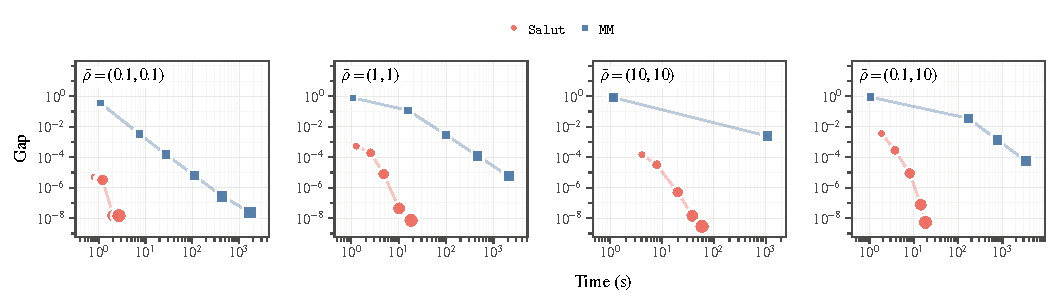
\includegraphics[width=\linewidth]{figures/uot_l2_accuracy_runtime_pareto.pdf}
\caption{\textbf{Runtime--accuracy comparison with $\ell_2^2$ marginal penalties.}
Runtime versus \sharedgap at $m=n=32{,}768$.
Larger markers target higher accuracy.}
\label{fig:l2-runtime-accuracy}
\end{figure}

Figure~\ref{fig:l2-generality} compares \ours and \mm across three additional ground costs under $\ell_2^2$ marginal penalties.
Across all three costs, \ours reaches mean gaps below $6.3\times10^{-9}$ within $8.9$ seconds.

\begin{figure}[htbp]
\centering
% CN: 完整五 seed 汇总、图源和校验和见 figures/plot_sources/l2_generality_20261118.json；150 个有效测量形成 30 个均值点。
% EN: Complete five-seed aggregates, figure sources and checksums: figures/plot_sources/l2_generality_20261118.json; 150 valid measurements form 30 mean points.
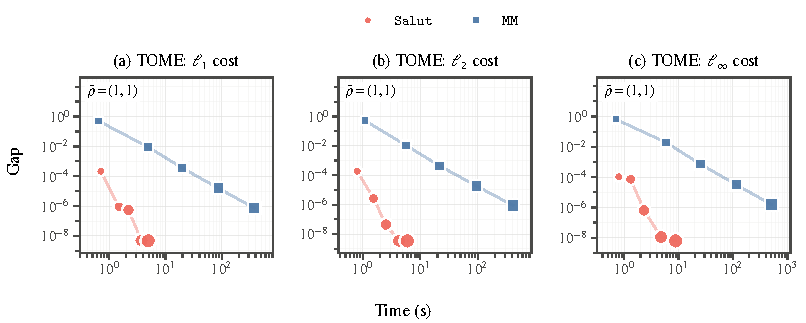
\includegraphics[width=0.76077\linewidth]{figures/uot_l2_generality.pdf}
\caption{\textbf{Ground-cost generality with $\ell_2^2$ marginal penalties.}
Runtime versus \sharedgap with $\ell_1$, $\ell_2$, and $\ell_\infty$ ground costs ($m=n=16{,}384$).
Larger markers target higher accuracy; points average five random seeds.}
\label{fig:l2-generality}
\end{figure}

Figure~\ref{fig:l2-scaling} evaluates scaling to million-point MERFISH instances.
At $m=n=1{,}048{,}576$, mean runtimes range from $148$ to $889$ seconds across the four penalty settings, with mean peak memory below $6.80$ GiB and mean gaps below $4.9\times10^{-5}$.

\begin{figure}[htbp]
\centering
% CN: 五 seed 完整结果见 figures/plot_sources/l2_scaling_20261120.json；图中不画误差棒，曲线为五 seed 均值；原始异常记录保留在源 batch 的 retry_history/。
% EN: Complete five-seed results: figures/plot_sources/l2_scaling_20261120.json; the plot omits error bars and shows five-seed means; original reviewed runs remain in the source batch's retry_history/.
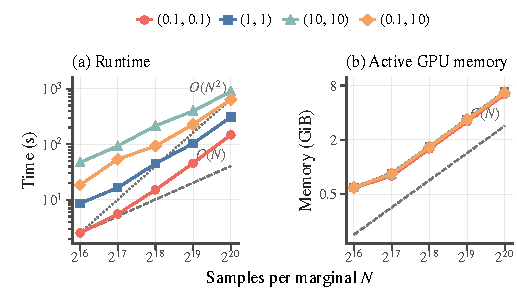
\includegraphics[width=3.45in]{figures/uot_l2_scaling.pdf}
\caption{\textbf{Scaling with $\ell_2^2$ marginal penalties.}
Runtime and peak GPU memory on MERFISH across sample sizes.
Legend entries give $(\bar\rho_a,\bar\rho_b)$; gray lines indicate reference slopes.
Markers show five-seed means.}
\label{fig:l2-scaling}
\end{figure}
